\documentclass[runningheads]{llncs}



\usepackage{enumitem}


\usepackage{color}

\usepackage{graphicx}
\usepackage{tikz}
\usepackage{calc}
\usepackage{array}

\usepackage{amsmath, amssymb}
\DeclareMathOperator*{\argmin}{arg\,min}

\usepackage{graphbox}
\usepackage{wasysym}

\usetikzlibrary{automata,arrows}

\usepackage{comment}

\usepackage{wrapfig}

\usepackage{hyperref}


\title{Counting infinitely by oritatami co-transcriptional folding}

%\titlerunning{}
\author{
Kohei Maruyama\inst{1}\and
Shinnosuke Seki\inst{1,2}
}
\institute{
The University of Electro-Communications, 
%Graduate School of Informatics and Engineering, 
1-5-1 Chofugaoka, Chofu, Tokyo, 1828585, Japan \email{\{k.maruyama, s.seki\}@uec.ac.jp}\and
\'{E}cole Normale Superi\'{e}ure de Lyon, 46 all\'{e}e d'Italie, 69007, Lyon, France
}

\begin{document}

\maketitle

\begin{abstract}
A fixed bit-width counter was proposed as a proof-of-concept demonstration of an oritatami model of cotranscriptional folding [Geary et al., Proc.~MFCS 2016, LIPIcs 58, 43:1-43:14], and it was embedded into another oritatami system that self-assembles a finite portion of Heighway dragon fractal. 
In order to expand its applications, we endow this counter with capability to widen bit-width at every encounter with overflow. 
\end{abstract}

%------------------------------------------------------
	\section{Introduction}
%------------------------------------------------------

Counting is one of the most essential tasks for computing; as well known, it suffices to count for Turing universality \cite{Minsky1967}. 
Nature has been counting billions of days using molecular ``circadian clockwork'' which is ``as complicated and as beautiful as the wonderful chronometers developed in the 18th century''  \cite{McClung2006}. 
Nowadays, developments in molecular self-assembly technology enable us to design molecules to count. 
Evans has recently demonstrated a DNA tile self-assembly system that counts accurately in binary from a programmed initial count until it overflows \cite{EvansPhD}. 
In its foundational theory of molecular self-assembly, such binary counters have proved their versatility, being used to assemble shapes of particular size \cite{AdChGoHu2001,RothemundWinfree2000}, towards self-assembly of fractals \cite{MasudaSekiUbukata2018}, as an infinite scaffold to simulate all Turing machines in parallel in order to prove undecidability of nondeterminism in the abstract tile-assembly model \cite{BrChDoKaSe2013}, to name a few. 

\begin{figure}[tb]
\centering
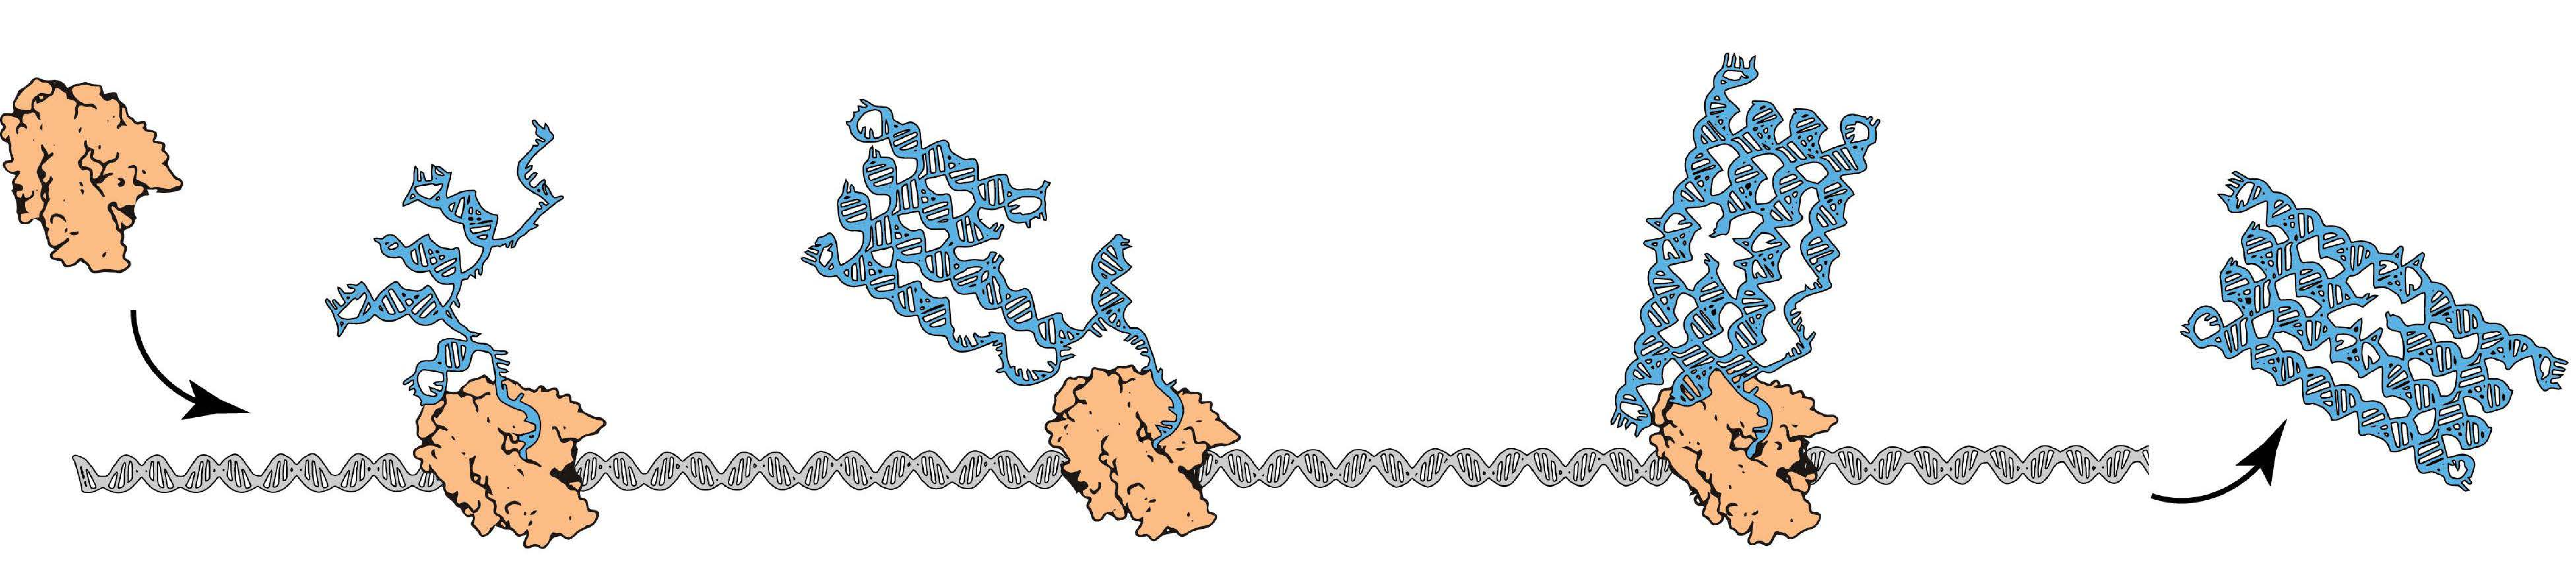
\includegraphics[width=\linewidth]{fig/rna_origami.pdf}
\caption{RNA origami}
\label{fig:rna_origami}
\end{figure}

A fixed bit-width (finite) binary counter has been implemented as a proof-of-concept demonstration of oritatami model of cotranscriptional folding \cite{GeMeScSe2019}. 
As shown in Fig.~\ref{fig:rna_origami}, an RNA transcript folds upon itself while being transcribed (synthesized) from its corresponding DNA template strand. 
Geary et al. programmed a specific RNA rectangular tile structure into a DNA template in such a way that the corresponding RNA transcript \textit{folds cotranscriptionally} into the programmed tile structure highly likely \textit{in vitro} at room temperatures (\textit{RNA origami}) \cite{GearyRothemundAndersen2014}. 
An oritatami system folds a transcript of abstract molecules called \textit{beads} of finitely many types cotranscriptionally over the 2-dimensional triangular lattice cotranscriptionally according to a rule set that specifies which types of molecules are allowed to bind. 
The transcript of the binary counter in \cite{GeMeScSe2019} is of period 60 as $\textcircled{\scriptsize 0}{-}\textcircled{\scriptsize 1}{-}\textcircled{\scriptsize 2}{-} \cdots {-}\textcircled{\scriptsize 58}{-}\textcircled{\scriptsize 59}{-}\textcircled{\scriptsize 0}{-}\textcircled{\scriptsize 1} \cdots$ and its period is semantically divided into two half-adder (HA) modules $A = \textcircled{\scriptsize 0}{-}\textcircled{\scriptsize 1}{-} \cdots {-}\textcircled{\scriptsize 11}$ and $C = \textcircled{\scriptsize 30}{-}\textcircled{\scriptsize 31}{-} \cdots {-}\textcircled{\scriptsize 41}$ and two structural modules $B$ and $D$, which are sandwiched by half-adder modules.
While being folded cotranscriptionally in zigzags, HA modules increment the current count $i$ by 1, which is initialized on a linear \textit{seed} structure, alike the Evans' counter, whereas structural modules $B$ and $D$ align HA modules properly and also make a turn at an end of the count $i$; $B$ guides the transcript from a zig to a zag ($\hookrightarrow$) while $D$ does from a zag to a zig ($\hookleftarrow$). 
This counter was embedded as a component of an oritatami system to self-assemble an arbitrary finite portion of Heighway dragon fractal \cite{MasudaSekiUbukata2018}. 
Its applications are limited, however, by lack of mechanism to widen bit-width; its behavior is undefined when its count overflows. 
In this paper, we endow this counter, or more precisely, its structural module $B$, with capability to widen the count by 1 bit at every encounter with overflow. 




%Our body consists many proteins which is based on genetic sequence in DNA.
%DNA sequence has to be copied in order to make proteins because DNA is in cell nucleus.
%It is copied to RNA (and its sequence is called \textit{transcript}) by a RNA polymerase and delivered to out of nucleus.
%A transcript consists four types nucleobases A, U, G, and C, and a nucleobase are called \textit{bead}
%Moreover, they form hydrogen bonds mainly between A and U, and between G and C, then they begin to form at the same time synthesizing.
%Once the bead is fixed after that it can not change the position.
%By repeating this method, transcript form a 3D shape.
%
%A shape of RNA depends on the DNA sequence.
%Geary, Rothemund, and Andrsen have succeeded in experimentally making 2D RNA tiles (Fig.\ref{fig:rna_origami}) by repeatedly copying a specific DNA sequence \cite{GearyRothemundAndersen2014}.
%Then, Oritatami System was designed as a mathematical model that the process of RNA production \cite{counter2016} and Fig.\ref{fig:origami_on_oritatami} is the 2D RNA tile which is represented on Oritatami System.
%Oritatami system treats transcript and nucleobase as paths and vertices which called \textit{bead}, respectively, moreover, they are arranged on a triangular grid.
%The system takes transcript as an input and output an terminal conformation.
%Geary et al. implemented binary counter in this system \cite{counter2016}.
%This counter is folded in zigzags, and each row represents a counted number.
%Then, this counter is given a bit width as an input to the system before transfer begins, and encounters nondeterminism if it carries beyond that bit width.
%Since it is running on deterministic system, it halts when it becomes nondeterministic.
%
%In this paper, based on the implementation method of this counter, we implement a counter which defined the behavior that extends the bit width when it overflows.



%\begin{figure}[tb]
%\centering
%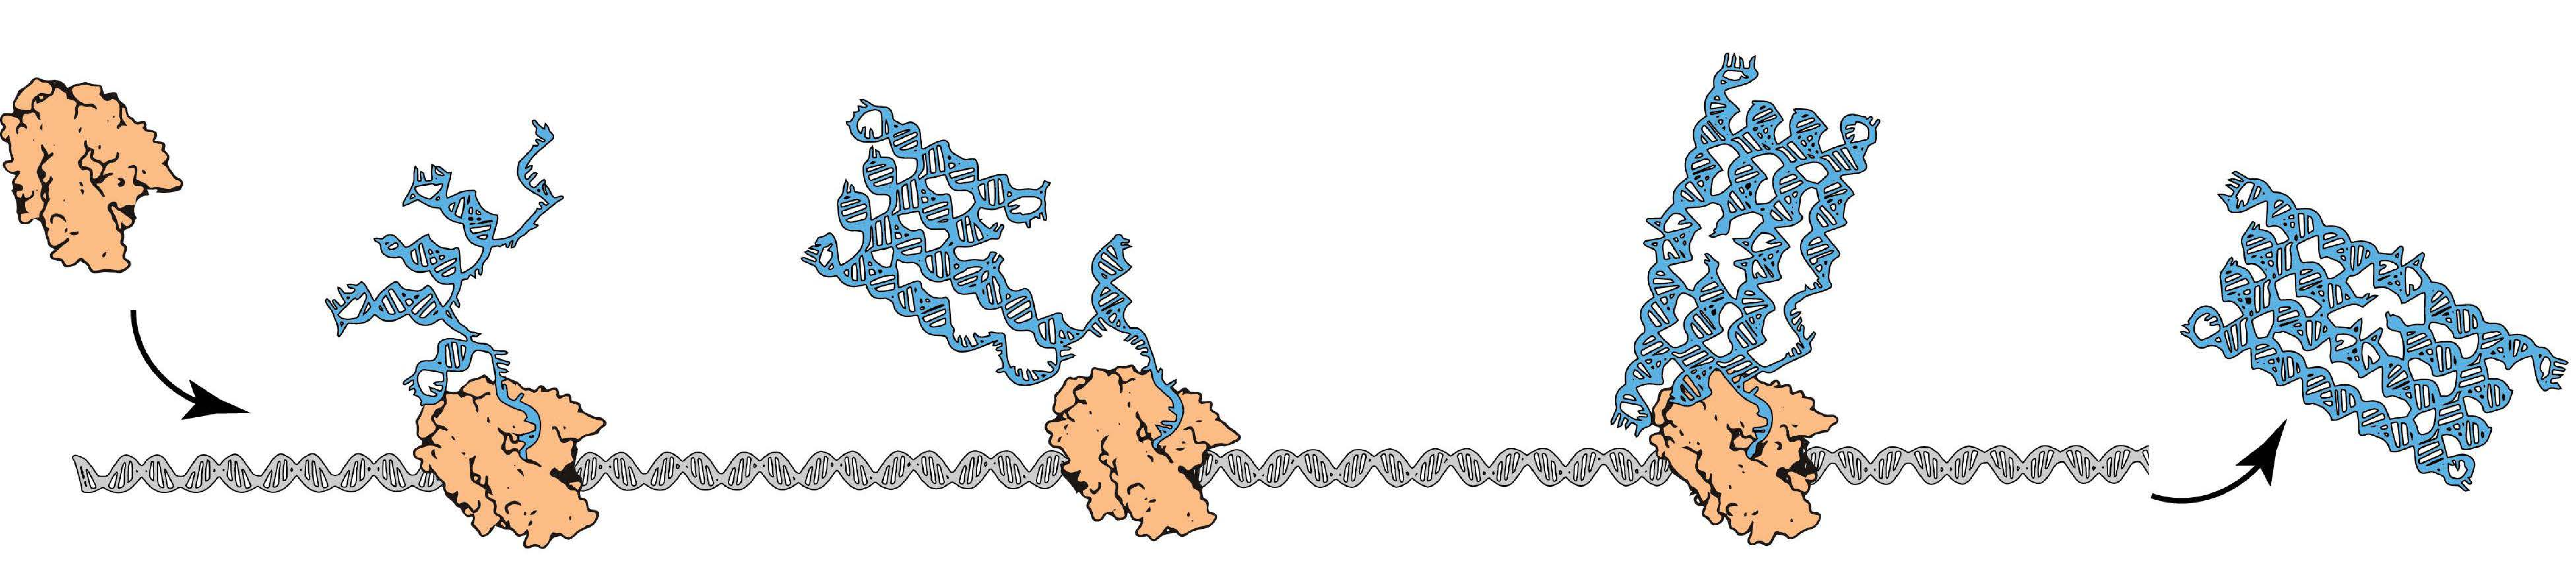
\includegraphics[width=\linewidth]{fig/rna_origami.pdf}
%\caption{
%A generated and stabilized 2D RNA tile from DNA
%}
%\label{fig:rna_origami}
%\end{figure}
%
%\begin{figure}[tb]
%\centering
%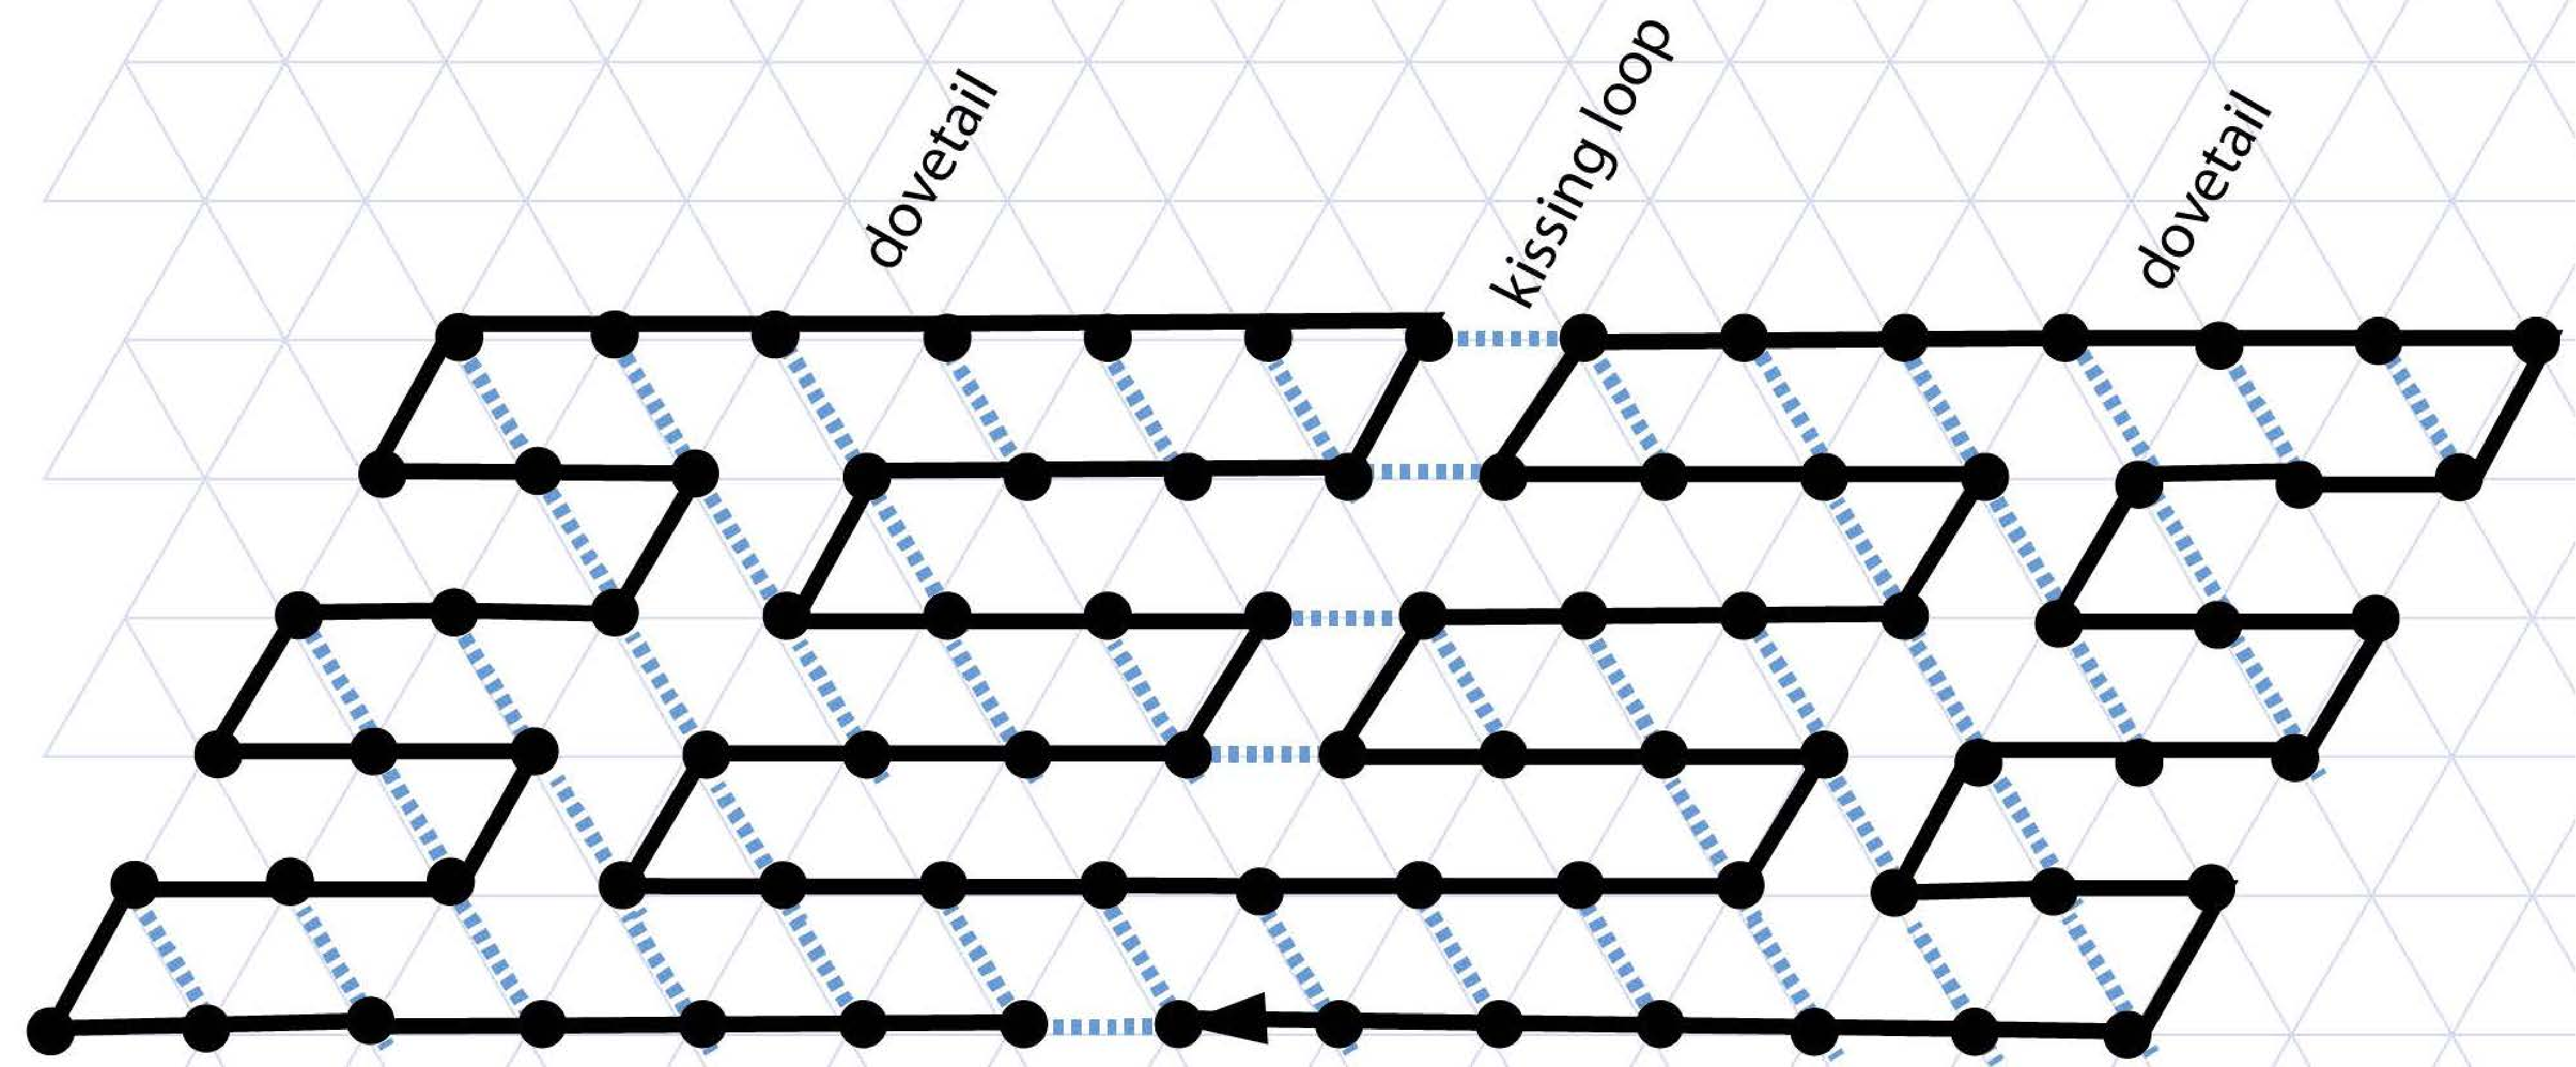
\includegraphics[width=\linewidth]{fig/origami_oritatami.pdf}
%\caption{
%The represented 2D RNA tile on Oritatami System
%}
%\label{fig:origami_on_oritatami}
%\end{figure}



%------------------------------------------------------
	\section{Preliminaries}
%------------------------------------------------------

%copy from TAMC2019 paper

Let $\Sigma$ be a finite alphabet, whose element should be regarded as type of abstract molecule, or \textit{beads}. 
A bead of type $a \in \Sigma$ is called an $a$-bead. 
By $\Sigma^*$ and $\Sigma^\omega$, we denote the set of finite sequences of beads and that of one-way infinite sequences of beads, respectively. 
The empty sequence is denoted by $\lambda$. 
Let $w = b_1 b_2 \cdots b_n \in \Sigma^*$ be a sequence of length $n$ for some integer $n$ and bead types $b_1, \ldots, b_n \in \Sigma$. 
The \textit{length} of $w$ is denoted by $|w|$, that is, $|w| = n$. %ここから要らない?↓やっぱり要る
For two indices $i, j$ with $1 \le i \le j \le n$, we let $w[i..j]$ refer to the subsequence $b_i b_{i+1} \cdots b_{j-1}b_j$; if $i = j$, then $w[i..i]$ is simplified as $w[i]$. 
For $k \ge 1$, $w[1..k]$ is called a \textit{prefix} of $w$. 

Oritatami systems fold their transcript, which is a sequence of beads, over the triangular grid graph $\mathbb{T} = (V, E)$ cotranscriptionally. %↓
For a point $p \in V$, let $\hexagon_p^d$ denote the set of points which lie in the regular hexagon of radius $d$ centered at the point $p$. 
Note that $\hexagon_p^d$ consists of $3d(d+1)+1$ points. %←
A directed path $P = p_1 p_2 \cdots p_n$ in $\mathbb{T}$ is a sequence of \textit{pairwise-distinct} points $p_1, p_2, \ldots, p_n \in V$ such that $\{p_i, p_{i+1}\} \in E$ for all $1 \le i < n$. 
Its $i$-th point is referred to as $P[i]$. 
Now we are ready to abstract RNA single-stranded structures in the name of conformation. 
A \textit{conformation} $C$ (over $\Sigma$) is a triple $(P, w, H)$ of a directed path $P$ in $\mathbb{T}$, $w \in \Sigma^*$ of the same length as $P$, and a set of h-interactions $H \subseteq \bigl\{\{i, j\} \bigm| 1 \le i, i+2 \le j, \{P[i], P[j]\} \in E \bigr\}$. 
This is to be interpreted as the sequence $w$ being folded along the path $P$ in such a manner that its $i$-th bead $w[i]$ is placed at the $i$-th point $P[i]$ and the $i$-th and $j$-th beads are bound (by a hydrogen-bond-based interaction) if and only if $\{i, j\} \in H$. 
The condition $i+2 \le j$ represents the topological restriction that two consecutive beads along the path cannot be bound. 
The \textit{length} of $C$ is defined to be the length of its transcript $w$ (that is, equal to the length of the path $P$). 
A \textit{rule set} $R \subseteq \Sigma \times \Sigma$ is a symmetric relation over $\Sigma$, that is, for all bead types $a, b \in \Sigma$, $(a, b) \in R$ implies $(b, a) \in R$.
A bond $\{i, j\} \in H$ is \textit{valid with respect to $R$}, or simply $R$-valid, if $(w[i], w[j]) \in R$. 
This conformation $C$ is \textit{$R$-valid} if all of its bonds are $R$-valid. %↓
For an integer $\alpha \ge 1$, $C$ is \textit{of arity $\alpha$} if it contains a bead that forms $\alpha$ bonds but none of its beads forms more. 
By $\mathcal{C}_{\le \alpha}(\Sigma)$, we denote the set of all conformations over $\Sigma$ whose arity is at most $\alpha$; its argument $\Sigma$ is omitted whenever $\Sigma$ is clear from the context. 

The oritatami system grows conformations by an operation called elongation. 
Given a rule set $R$ and an $R$-valid conformation $C_1 = (P, w, H)$, we say that another conformation $C_2$ is an elongation of $C_1$ by a bead $b \in \Sigma$, written as $C_1 \xrightarrow{R}_b C_2$, if $C_2 = (P p, wb, H \cup H')$ for some point $p \in V$ not along the path $P$ and set $H' \subseteq \bigl\{ \{i, |w|+1\} \bigm| 1 \le i < |w|, \{P[i], p\} \in E, (w[i], b) \in R \bigr\}$ of bonds formed by the $b$-bead; this set $H'$ can be empty. 
Note that $C_2$ is also $R$-valid. 
This operation is recursively extended to the elongation by a finite sequence of beads as: for any conformation $C$, $C \xrightarrow{R}_\lambda^* C$; and for a finite sequence of beads $w \in \Sigma^*$ and a bead $b \in \Sigma$, a conformation $C_1$ is elongated to a conformation $C_2$ by $wb$, written as $C_1 \xrightarrow{R}_{wb}^* C_2$, if there is a conformation $C'$ that satisfies $C_1 \xrightarrow{R}_w^* C'$ and $C' \xrightarrow{R}_b C_2$. 

An \textit{oritatami system} (OS) $\Xi$ is a tuple $(\Sigma, R, \delta, \alpha, \sigma, w)$, where $\Sigma$ and $R$ are defined as above, while
\begin{itemize}
\item a positive integer $\delta$ called \textit{delay}, 
\item a positive integer $\alpha$ called \textit{arity}, %←arityの行だけ要らない?
\item an initial $R$-valid conformation $\sigma \in C_{\le \alpha}(\Sigma)$ called the \textit{seed},
\item a (possibly infinite) \textit{transcript} $w \in \Sigma^* \cup \Sigma^\omega$, which is to be folded upon the seed by stabilizing beads of $w$ one at a time so as to minimize energy collaboratively with the succeeding $\delta{-}1$ nascent beads. 
\end{itemize}
%
The energy of a conformation $C = (P, w, H)$, denoted by $\Delta G(C)$, is defined to be ${-}|H|$; the more bonds a conformation has, the more stable it gets. 
The set $\mathcal{F}(\Xi)$ of conformations \textit{foldable} by the system $\Xi$ is recursively defined as: the seed $\sigma$ is in $\mathcal{F}(\Xi)$; and provided that an elongation $C_i$ of $\sigma$ by the prefix $w[1..i]$ be foldable (i.e., $C_0 = \sigma$), its further elongation $C_{i+1}$ by the next bead $w[i+1]$ is foldable if 
\begin{equation}\label{eq:OS_CF}
C_{i+1} \in \argmin_{
\substack{
C \in \mathcal{C}_{\le \alpha} s.t. \\
C_i \xrightarrow{R}_{w[i+1]}C \\
}
}
\min \Bigl\{ \Delta G(C') \Bigm|
C \xrightarrow{R}^*_{w[i+2...i+k]}C', k\le \delta, C' \in \mathcal{C}_{\le \alpha}
\Bigr\}.
\end{equation}
%
Then we say that the bead $w[i+1]$ and the bonds it forms are \textit{stabilized} according to $C_{i+1}$. 
The easiest way to understand this stabilization process should be the video available at \href{https://www.dailymotion.com/video/x3cdj35}{\tt https://www.dailymotion.com/video/x3cdj35}, in which the Turing universal oritatami system by Geary et al. \cite{GeMeScSe2018}, whose delay is 3, is running. 
Note that an arity-$\alpha$ oritatami system cannot fold any conformation of arity larger than $\alpha$. %←
A conformation foldable by $\Xi$ is \textit{terminal} if none of its elongations is foldable by $\Xi$. 
%The oritatami system $\Xi$ is \textit{deterministic} if for all $i \ge 0$, there exists at most one $C_{i+1}$ that satisfies \eqref{eq:OS_CF}. 
%A deterministic oritatami system folds into a unique terminal conformation. 
%An oritatami system with the empty rule set just folds into an arbitrary elongation of its seed nondeterministically. 
%Thus, the rule set is reasonably assumed non-empty. 



\begin{figure}[tb]
\begin{tabular}{c}
 \begin{minipage}{0.5\linewidth}
  \centering
   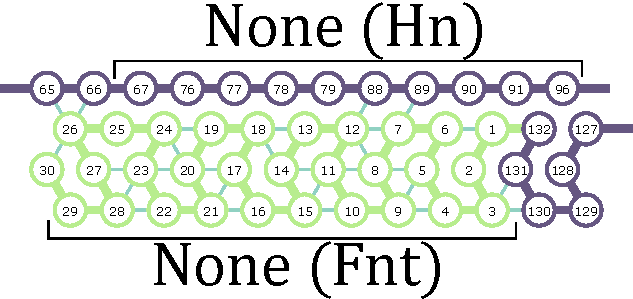
\includegraphics[width=0.8\linewidth]{fig/svg/Fnt_1.pdf}
 \end{minipage}
 
 \begin{minipage}{0.5\linewidth}
  \centering
   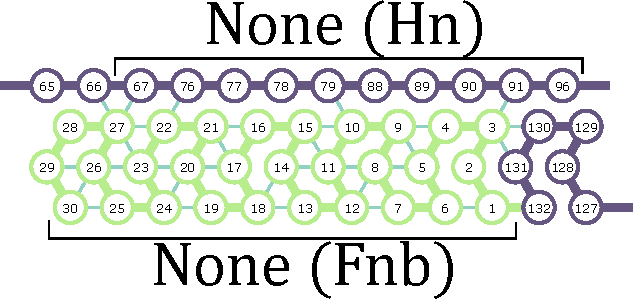
\includegraphics[width=0.8\linewidth]{fig/svg/Fnb_1.pdf}

 \end{minipage}
 \end{tabular}
\ \\
\ \\
\begin{tabular}{c}
 \begin{minipage}{0.5\linewidth}
  \centering
   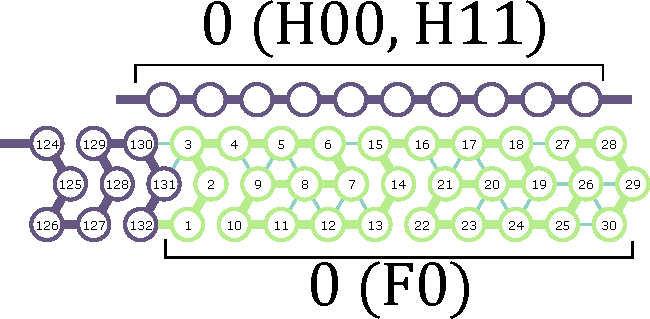
\includegraphics[width=0.8\linewidth]{fig/svg/F0_1.pdf}
 \end{minipage}
 
 \begin{minipage}{0.5\linewidth}
  \centering
   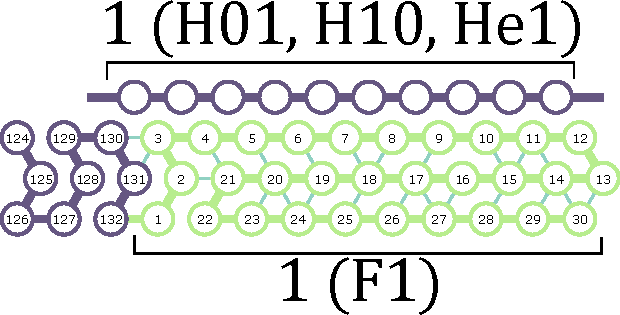
\includegraphics[width=0.8\linewidth]{fig/svg/F1_1.pdf}

 \end{minipage}
 \end{tabular}
 \caption{All the four bricks of module F: The two bricks at the top, \texttt{Fnt} and \texttt{Fnb}, are for zigs while the others, \texttt{F0} and \texttt{F1}, are for zags. }
 \label{fig:formatters}
\end{figure}

\begin{figure}[tb]
\begin{tabular}{c}
 \begin{minipage}{0.5\linewidth}
  \centering
   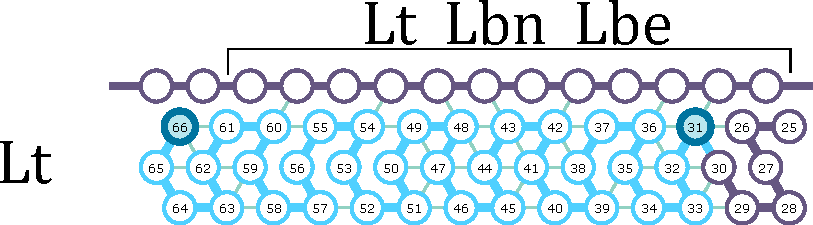
\includegraphics[width=0.9\linewidth]{fig/svg/Lt_3.pdf}
 \end{minipage}
 
 \begin{minipage}{0.5\linewidth}
  \centering
   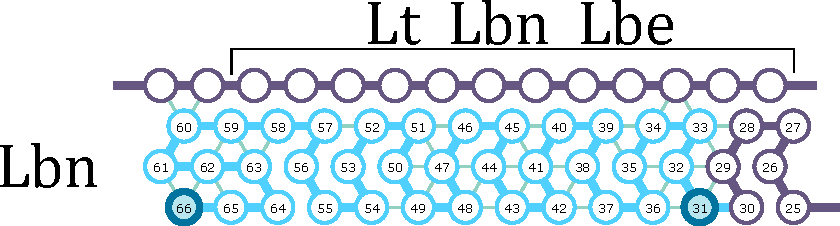
\includegraphics[width=0.9\linewidth]{fig/svg/Lbc_3.pdf}

 \end{minipage}
 \end{tabular}

\ \\
\ \\
  \centering
   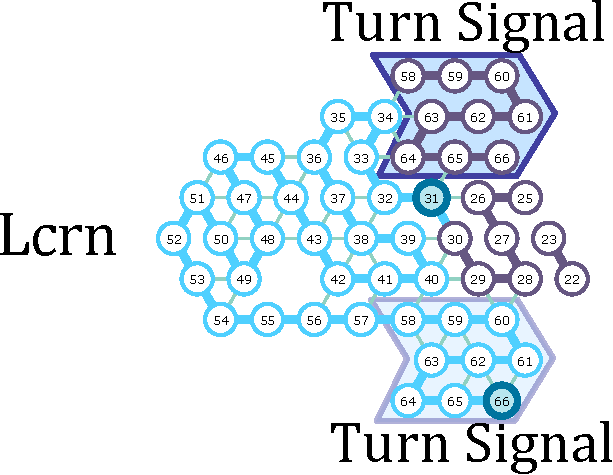
\includegraphics[width=0.4\linewidth]{fig/svg/Ltrc_3.pdf}


\begin{tabular}{c}
\ \\
\ \\
 \begin{minipage}{0.5\linewidth}
  \centering
   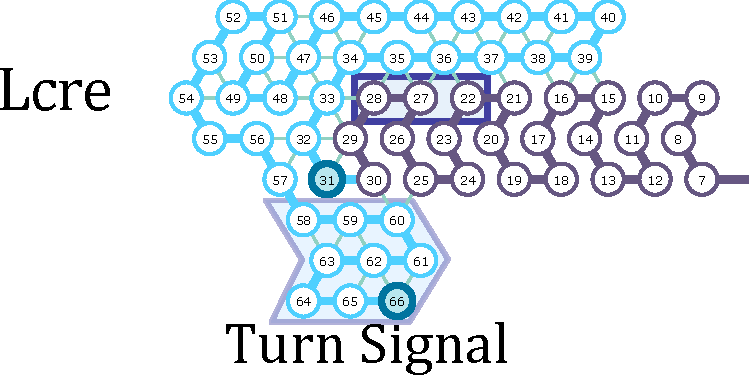
\includegraphics[width=0.9\linewidth]{fig/svg/Ltre_3.pdf}
 \end{minipage}
 
  \begin{minipage}{0.5\linewidth}
  \centering
   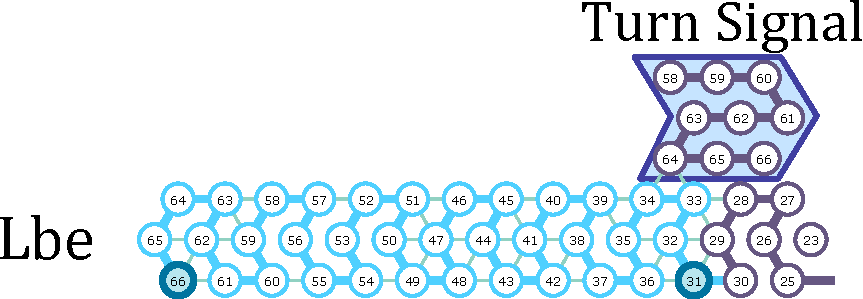
\includegraphics[width=\linewidth]{fig/svg/Lbe_3.pdf}
   \vspace*{18mm}

 \end{minipage}
 \end{tabular}
 \caption{All the five bricks of module L: \texttt{Lt}, \texttt{Lbn}, \texttt{Lcrn}, \texttt{Lcre}, and \texttt{Lbe} from top left to bottom right.
In zigs, L folds into either \texttt{Lt} or \texttt{Lbn} depending on where it starts, until the transcript reaches the left end, where L folds either into \texttt{Lcrn} if the current value has not been overflowed, or into \texttt{Lbe} at an overflow.
In the case of overflow, the next L folds into \texttt{Lcre}.
In zags, L always folds into \texttt{Lbn}.}
 \label{fig:leftturns}
\end{figure}


\section{Folding an infinite binary counter}

\subsection{General idea}
Between two consecutive overflows, the proposed system behaves in the same way as the finite binary counter proposed by Geary et al. \cite{GeMeScSe2019}.
Its transcript folds in a zigzag manner macroscopically (downward in figures throughout this paper).
A zig, folding from right to left, increments the current value of the counter by 1.
The succeeding zag, folding from left to right, formats the incremented value for the sake of next zig and copies it downward.
Unlike the existing counter, when a zig encounters an overflow, it does not abort but rather extends the current value by 1 bit.

%Each zig or zag is 3-rows thick.
%Each pass extends to straight while folding into glider and folds its last module folds into turn module and starts next pass.


The transcript of our counter is periodic.
Its period 1-2-3- $\cdots$ -132 is semantically divided into the following 4 subsequences, called \textit{modules}:
\begin{itemize}
\item 1--30: Format module or F
\item 31--66: Left-Turn module or L
\item 67--96: Half-Adder module or H
\item 97--132: Right-Turn module  or R
\end{itemize}
The transcript can be hence represented as $(FLHR)^*$ at the module level. Modules are to play their roles in expected environments by folding into respective conformations which should be pairwise-distinct enough to be distinguishable by other modules transcribed later.
Such expected conformations are called a \textit{brick}.
For example, module F encounters only the four environments shown in Fig.~\ref{fig:formatters} where it takes the four bricks, respectively.

\begin{figure}[tb]
\begin{tabular}{c}
 \begin{minipage}{0.33\linewidth}
  \centering
   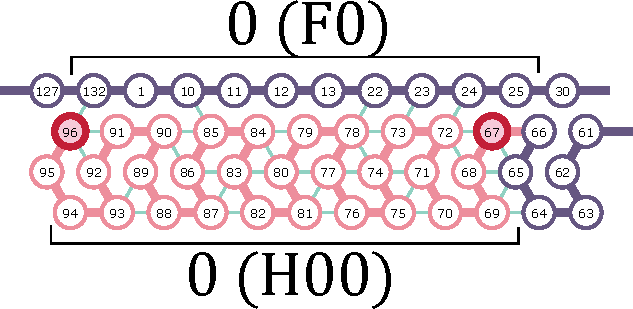
\includegraphics[width=0.9\linewidth]{fig/svg/H00_1.pdf}
 \end{minipage}
 
 \begin{minipage}{0.33\linewidth}
  \centering
   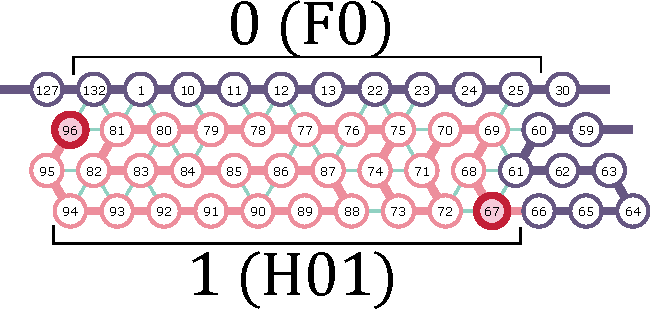
\includegraphics[width=0.9\linewidth]{fig/svg/H01_1.pdf}

 \end{minipage}
 
  \begin{minipage}{0.33\linewidth}
  \centering
   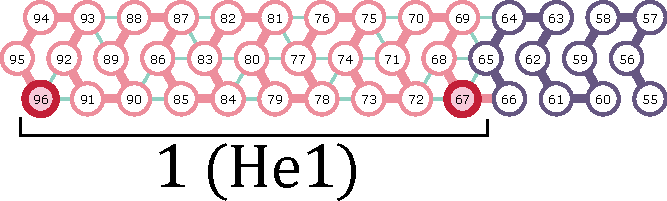
\includegraphics[width=0.9\linewidth]{fig/svg/He1_1.pdf}
 \end{minipage}
 \end{tabular}

\begin{tabular}{c}
\ \\
 \begin{minipage}{0.33\linewidth}
  \centering
   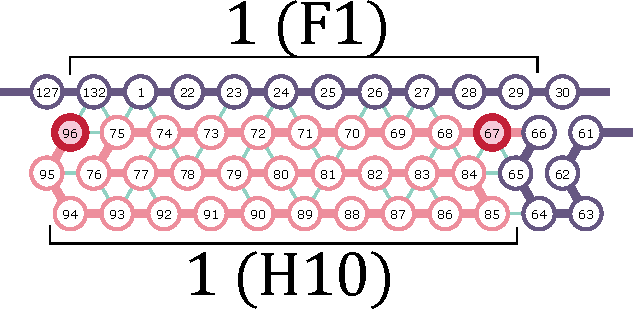
\includegraphics[width=0.9\linewidth]{fig/svg/H10_1.pdf}
 \end{minipage}
 
 \begin{minipage}{0.33\linewidth}
  \centering
   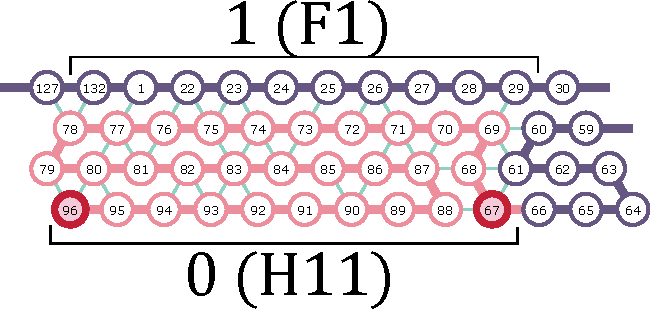
\includegraphics[width=0.9\linewidth]{fig/svg/H11_1.pdf}
 \end{minipage}
 
  \begin{minipage}{0.33\linewidth}
  \centering
   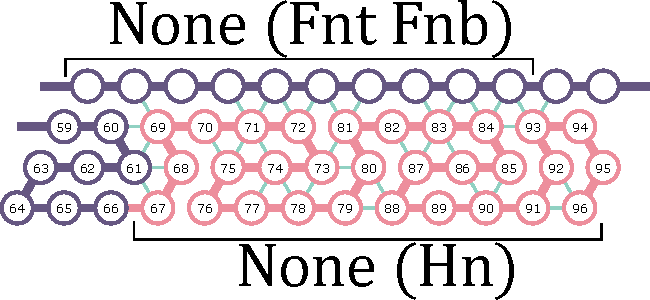
\includegraphics[width=0.9\linewidth]{fig/svg/Hn_1.pdf}

 \end{minipage}
 \end{tabular}
 \caption{All the six bricks of module H: \texttt{H00}, \texttt{H01}, \texttt{He1}, \texttt{H10}, \texttt{H11}, and \texttt{Hn} from top left to bottom right.
In zags, H always folds into \texttt{Hn} while in zigs, it folds into one of the other five bricks.}
 \label{fig:halfadders}
\end{figure}


\begin{figure}[tb]
\begin{tabular}{c}
 \begin{minipage}{0.5\linewidth}
  \centering
   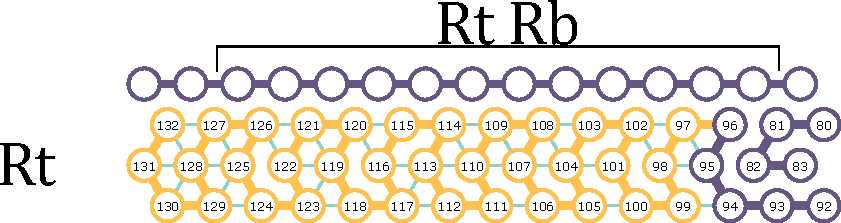
\includegraphics[width=0.8\linewidth]{fig/svg/Rt_1.pdf}
 \end{minipage}
 
 \begin{minipage}{0.5\linewidth}
  \centering
   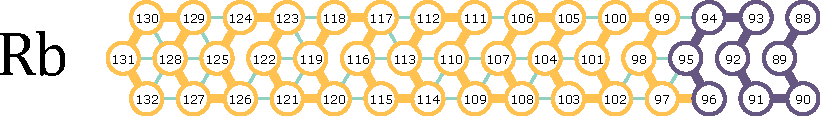
\includegraphics[width=0.8\linewidth]{fig/svg/Rb_1.pdf}

 \end{minipage}

\vspace{10mm}

\ \\
  \raggedright
   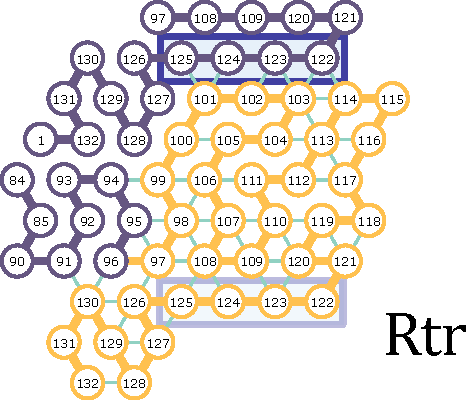
\includegraphics[width=0.3\linewidth]{fig/svg/Rtr_1.pdf}

 \end{tabular}
 \caption{All the three bricks of module R: \texttt{Rt}, \texttt{Rb}, and \texttt{Rcr}.
 In zigs, R folds into \texttt{Rt} or \texttt{Rb}.
 In zags, R always folds into \texttt{Rb} until the transcript reaches the right end, where R folds into \texttt{Rcr}.}
 \label{fig:rightturns}
\end{figure}

\paragraph{Seed and Encoding.}
The initial counter value is encoded as $b_{k-1}b_{k-2} \cdots b_1b_0$ in binary on the seed in the following format
\begin{equation} \label{eq:zagencoding}
64{-}65{-}66{-}\left( \prod^0_{i = k-1} \bigl(  w_{Hn} w_{Rb} w_{Fb_i} w_{Lbn} \bigr) \right) w_{Hn}
\end{equation}
where $w_{Hn}= 67{-}76{-}77{-}78{-}79{-}88{-}89{-}90{-}91{-}96$, $w_{Rb}=97{-}102{-}103{-}108{-}$ $109{-}114{-}115{-}120{-}121{-}126{-}127{-}132$, $w_{F0} = 1{-}10{-}11{-}12{-}13{-}22{-}23{-}24{-}$ $25{-}30$, $w_{F1}=1{-}22{-}23{-}24{-}25{-}26{-}27{-}28{-}29{-}30$, $w_{Lbn}= 31{-}36{-}37{-}42{-}$ $43{-}48{-}49{-}54{-}55{-}64{-}65{-}66$ are sequences of bead types exposed downward by modules H, R, F, L when they fold into bricks \texttt{Hn}, \texttt{Rb}, \texttt{F}$b_i$, \texttt{Lbn}, respectively, which can be found in Figs.~\ref{fig:halfadders}, \ref{fig:rightturns}, \ref{fig:formatters}, and \ref{fig:leftturns}.
For instance, the seed for $k = 1$ and $b_0 = 0$ is colored in purple in Fig.~\ref{fig:counter1stzig}.
%$w_{Hn} = 67{-}76{-}77{-}78{-}79{-}88{-}89{-}90{-}91{-}96$ \\
%$w_{Rb} = 97{-}102{-}103{-}108{-}109{-}114{-}115{-}120{-}121{-}126{-}127{-}132$\\
%$w_{Lbn} = 31{-}36{-}37{-}42{-}43{-}48{-}49{-}54{-}55{-}64{-}65{-}66$

\subsection{Brick level overview}
Starting from the seed, this system cyclically transits four phases: zig ($\leftarrow$), left carriage-return ($\hookrightarrow$), zag ($\rightarrow$), and right carriage-return ($\hookleftarrow$). 
The prefix $(FLHR)^k F$ of the transcript folds into the first zig (recall that $k$ is the bit-width of the initial value). 
In zigs in general, all the instances of modules F and H fold into bricks of width 10 and height 3, while all the instances of  L and R fold into bricks of width 12 and height 3. 
Zigs thus turn out to be a linear structure of height 3. 
In the process of the prefix folding into the first zig, its $i$-th instance of $H$ is transcribed right below $b_{i-1}$ encoded on the seed in the format (2) so that the H can ``read" $b_{i-1}$. 
After the whole prefix thus has folded into the first zig, the next L is transcribed right below Turn Signal, which lets the L fold into a special brick for left carriage-return if the zig ended at the top (this occurs when $b_{k-1} b_{k-2} \cdots b_0 < 1^k$) (see Fig.~\ref{fig:counter1stzag}). 
We should note that this special brick \texttt{Lcre} is provided with another Turn Signal for the sake of next left carriage-return.
Having been thus carriage-returned, the succeeding subsequence $(HRFL)^k H$ of the transcript folds into the first zag. 
Even in zags instances of F and H fold into bricks of width 10 and height 3, while those of L and R fold into bricks of width 12 and height 3. 
As a result, zags turn out to be a linear structure of height 3. 
More importantly, instances of H and F are aligned vertically and alternately into columns (see Figs.~\ref{fig:counter1stzig}-\ref{fig:overflowex1}), $i$-th of which from the right propagates the ($i{-}1$)-th bit of the counter value downward. 
After the whole subsequence has folded into the first zag, an instance of $R$ is transcribed and folded into a special brick \texttt{Rcr} for carriage-return due to the turn signal 125-124-123-122, which occurs also at the bottom of \texttt{Rcr} for the sake of next right carriage-return. 
This amounts to one cycle of the phase transition.

\subsubsection{In the zig ($\leftarrow$)} 
Here, the counter lets instances of module H increment its current value, which is encoded in the format \eqref{eq:zagencoding} below the seed or previous zag.
When the current value is $k$ bits in width, a subsequence $(FLHR)^kF$ of the transcript folds into the zig.
All the bricks which modules take in a zig are of height 3 (see Fig.~\ref{fig:formatters},  \ref{fig:halfadders}, \ref{fig:leftturns}, and \ref{fig:rightturns}) so that the zig turns out to be a linear structure of height 3.
Carry is propagated throughout the zig as a height for modules to start.
All modules but H end at the same height as it began, that is, do not change carry.
Module H can take the five bricks \texttt{H00}, \texttt{H01}, \texttt{H10}, \texttt{H11}, and \texttt{He1} shown in Fig.~\ref{fig:halfadders} in zigs but nothing else.
This is because the whole system is designed in such a way that module H encounters only the five environments.
Until the count overflows, module H encounters only four of them, which encode input 0 as $w_{F0}$ or 1 as $w_{F1}$ and carry or no-carry as the height for the module to start folding (bottom or top), where it takes \texttt{H00}, \texttt{H01}, \texttt{H10}, and \texttt{H11}, respectively, as shown in Fig.~\ref{fig:halfadders} (\texttt{H}$xc$ is folded when the input is $x$ and the carry is given if $c=1$ or not otherwise).

\begin{figure}[tb]
\centering
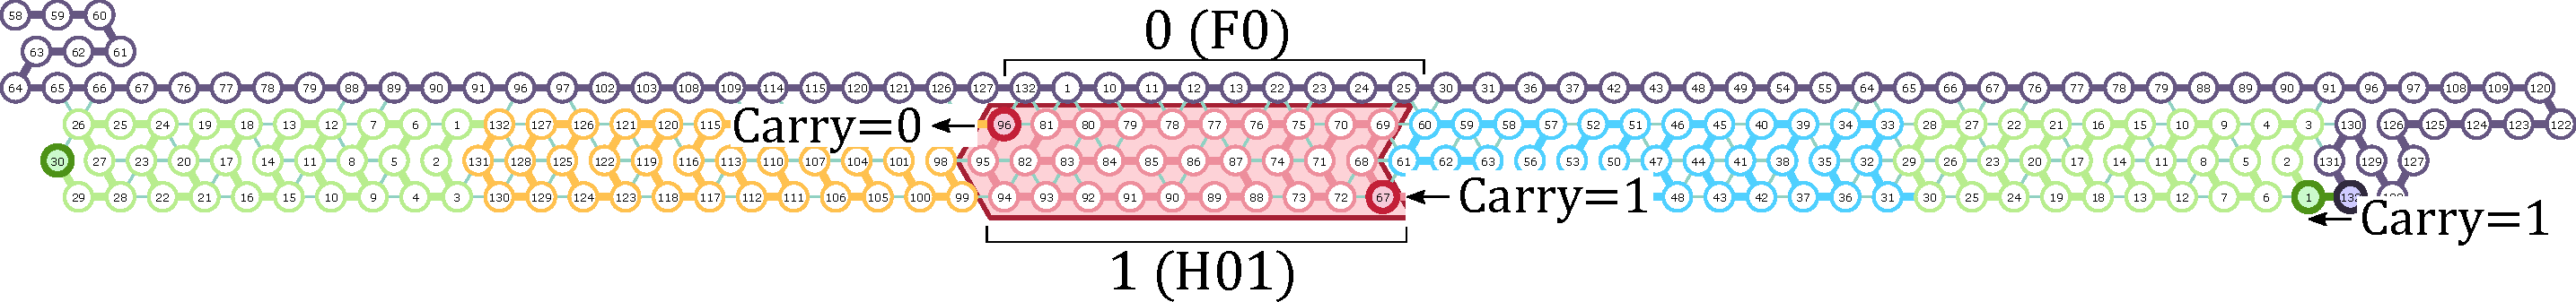
\includegraphics[width=\linewidth]{fig/svg/CounterEx5_1.pdf}
\caption{
The first zig.
0 is encoded as an initial value below the seed in the format \eqref{eq:zagencoding} with $k = 1$ (1-bit width).
Being fed with carry, the zig increments the value.
Module H outputs 1, or more precisely a sequence of bead types which shall be interpreted as 1 in the next zag and reformatted, as a sum and cancels the carry.
}
%\textcircled{\scriptsize 1}{-}\textcircled{\scriptsize 10}{-}\textcircled{\scriptsize 11}{-}\textcircled{\scriptsize 12}{-}\textcircled{\scriptsize 13}{-}\textcircled{\scriptsize 22}{-}\textcircled{\scriptsize 23}{-}\textcircled{\scriptsize 24}{-}\textcircled{\scriptsize 25}{-}\textcircled{\scriptsize 30},

\label{fig:counter1stzig}
\end{figure}

\begin{figure}[tb]
\centering
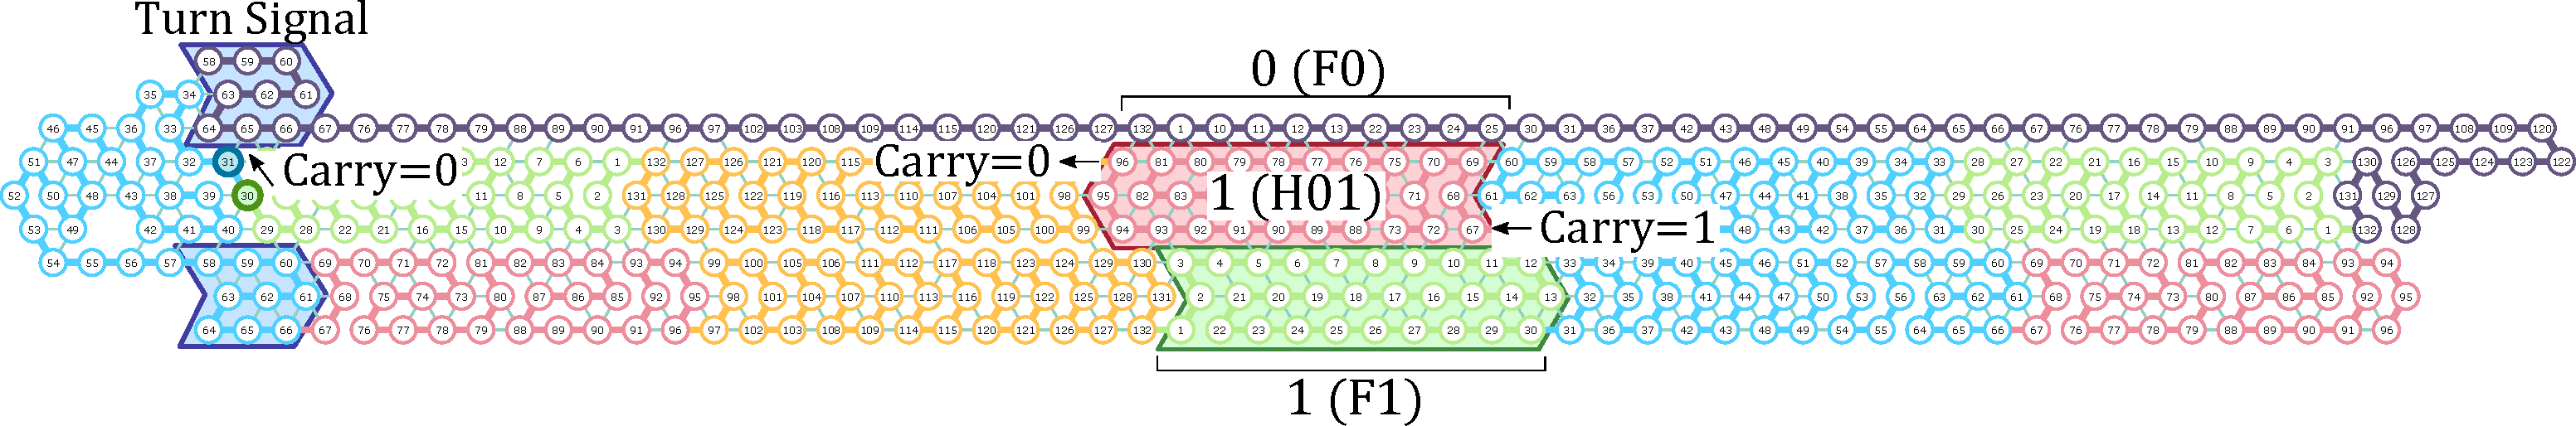
\includegraphics[width=\linewidth]{fig/svg/CounterEx11_1.pdf}
\caption{
Module L turns and start the first zag pass.
Since there is a Turn Signal at the left end of the seed, when the carry is 0, module L turns and at the end of L forms Turn Signal.
In zag pass, module F reads the output of module H and copies it down,
}
\label{fig:counter1stzag}
\end{figure}

\begin{figure}[tb]
\centering
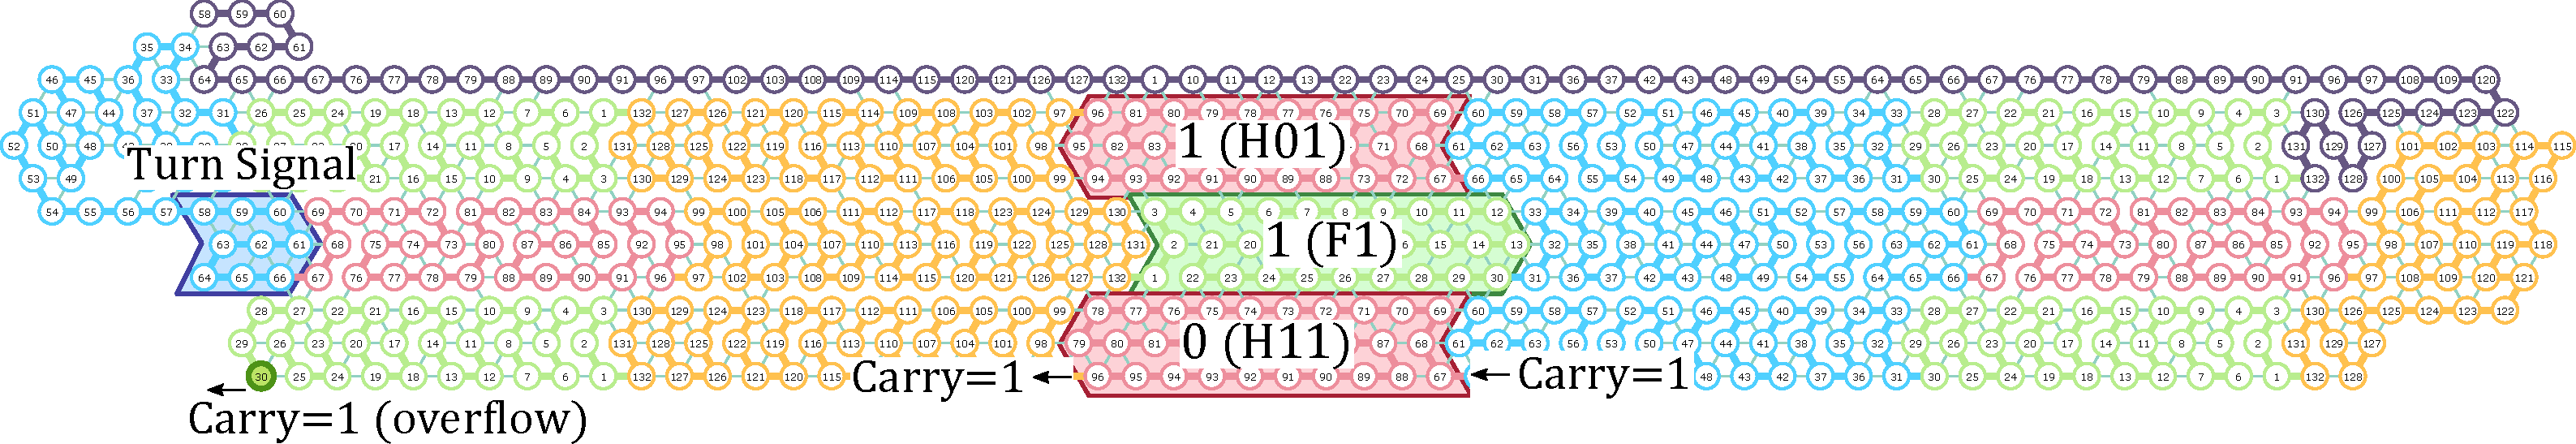
\includegraphics[width=\linewidth]{fig/svg/CounterEx13_1.pdf}
\caption{
Reach the left end with carry.
Even if transcript of module L sticks to Turn Signal, it can not bind because the distance is long.
}
\label{fig:overflowex1}
\end{figure}

Let us see how the subsequence $(FLHR)^kF$ folds into a zig; for $k=1$ and the current value 0, see Fig.~\ref{fig:counter1stzig}.
The zig is initially fed with carry by being forced to start folding at the bottom and the carry is propagated through the first instances of F and L in the way just explained toward the first instance of H.
This H is thus fed with carry and folds into \texttt{H01} if the bit encoded above is 0, as illustrated in Fig.~\ref{fig:counter1stzig}, or \texttt{H11} if the bit is rather 1.
\texttt{H01} ends at the top, corresponding to no-carry.
This absence of carry propagates through the succeeding modules leftward.
As a result, the zig ends, or more precisely an instance of F ends folding at the bottom if the current value is overflowed (Fig.~\ref{fig:overflowex1}), or at the top otherwise. (Fig.~\ref{fig:counter1stzig}).
An instance of L is to be transcribed next.
It folds either into \texttt{Lcrn} for (normal) carriage-return unless the current value is overflowed, or into \texttt{Lbe} at an overflow.

\subsubsection{In the zag ($\rightarrow$)}
Here, the value incremented in the previous zig is formatted so as to be exposed below in the format \eqref{eq:zagencoding} for the next zig.
A subsequence $(HRFL)^kH$ of the transcript folds into the zag, where $k$ is the bit width of the incremented value.
Both of the bricks of L for carriage-return, i.e., \texttt{Lcrn} and \texttt{Lcre}, ends at the bottom so that zags start at the bottom.
The first instances of H and R fold into \texttt{Hn} and \texttt{Rb}, respectively.
Hence, the next F starts at the bottom and takes the brick \texttt{F}$y$ under the module H  that takes the brick \texttt{H}$xc$ in the previous zig, where $y$ is the output of the module, that is, $y = (x+c) \mod 2$.
Both of these bricks \texttt{F0} and \texttt{F1} end at the bottom so that the instance of L folds into \texttt{Lbn}.


\begin{figure}[tb]
\centering
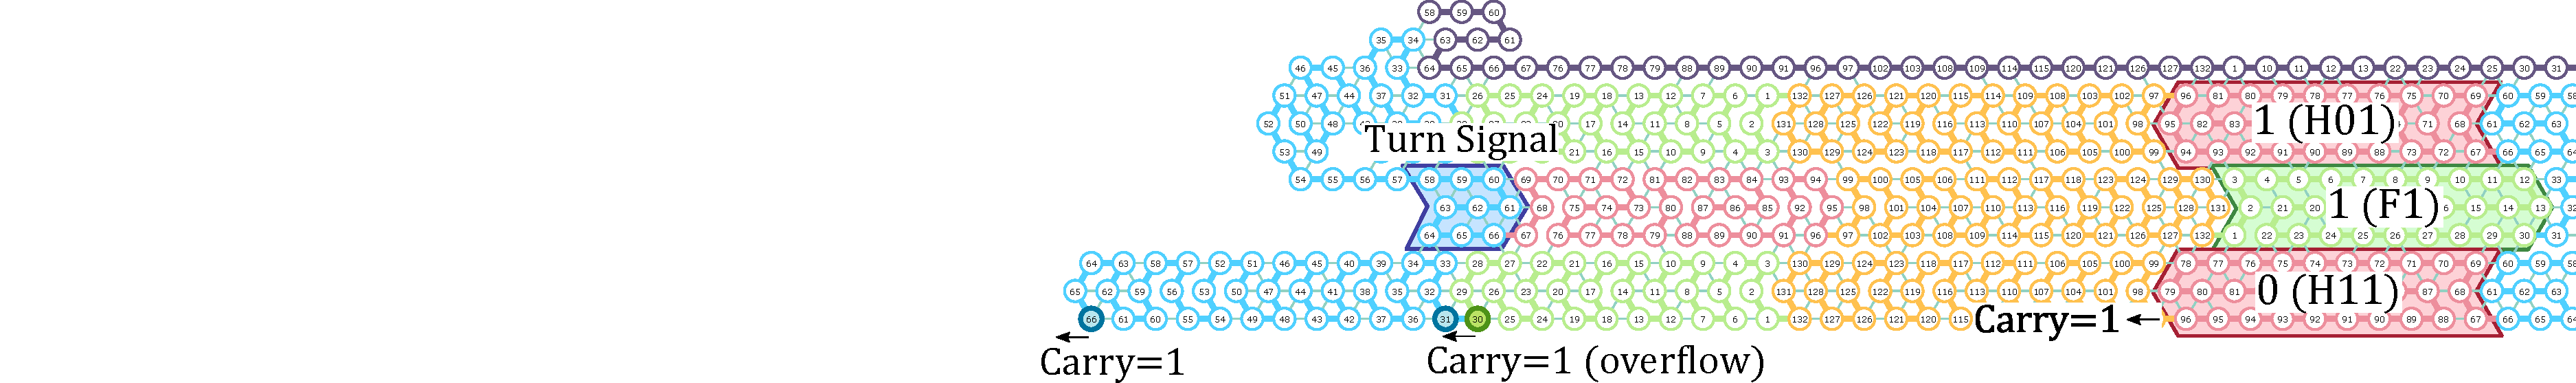
\includegraphics[width=\linewidth]{fig/svg/CounterEx14_1.pdf}
\caption{
Module L forms a glider shape without binding to Turn Signal and goes straight on. 
}
\label{fig:overflowex2}
\end{figure}

\begin{figure}[tb]
\centering
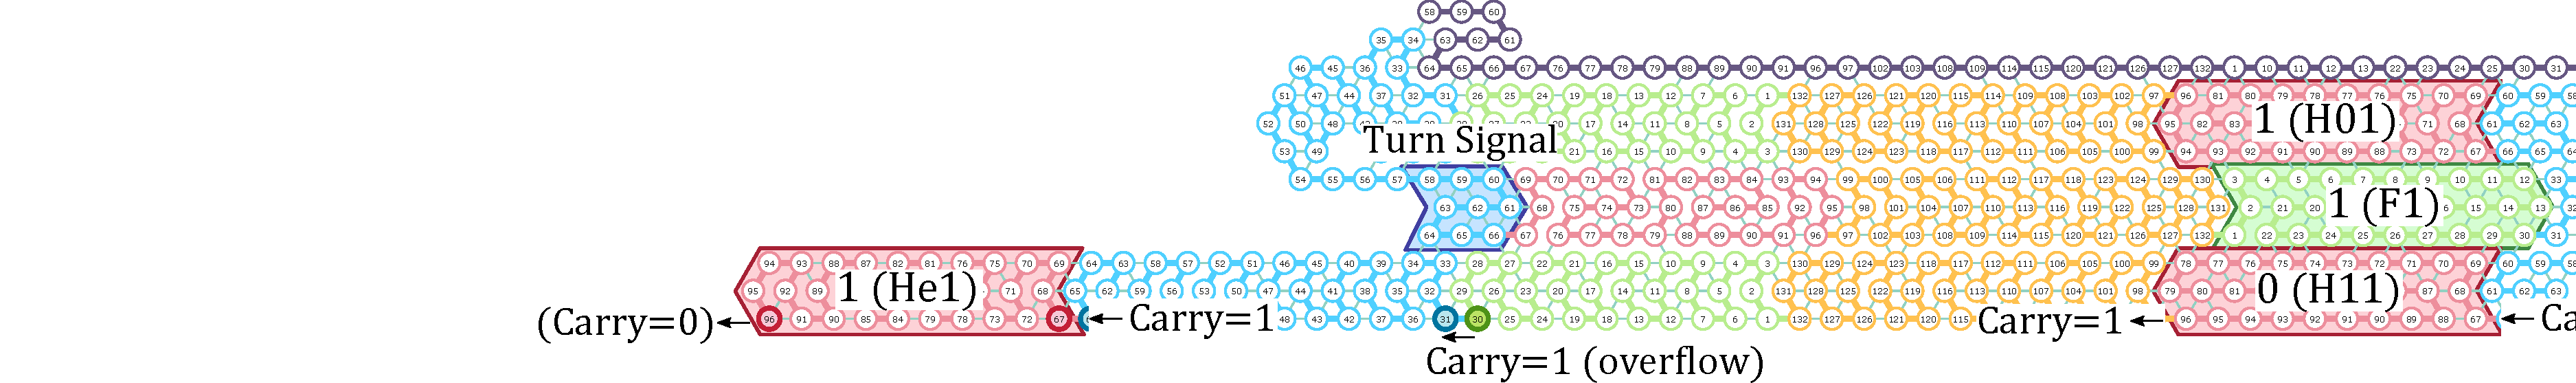
\includegraphics[width=\linewidth]{fig/svg/CounterEx15_1.pdf}
\caption{
Module H catches the overflowed carry but module H can not cancel the carry because it must be a self standing glider.
That is way the last bead of this module H is folded at the bottom but carry = 0. 
}
\label{fig:overflowex3}
\end{figure}


\begin{figure}[tb]
\centering
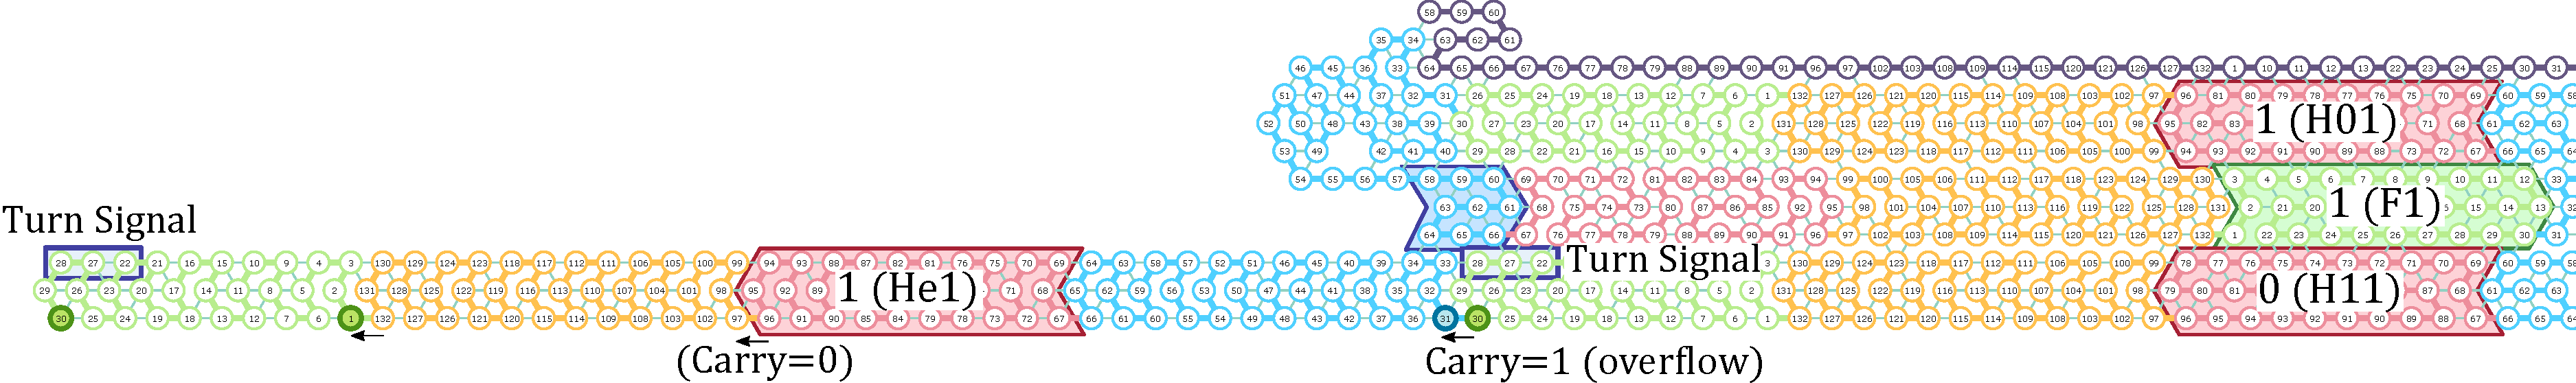
\includegraphics[width=\linewidth]{fig/svg/CounterEx17_1.pdf}
\caption{
Module R and F are folded, and then folding of module L starts, but without Turn Signal, L can not turn.
Then, turn module L by making the top of module F the Turn Signal.
}
\label{fig:overflowex4}
\end{figure}

\begin{figure}[tb]
\centering
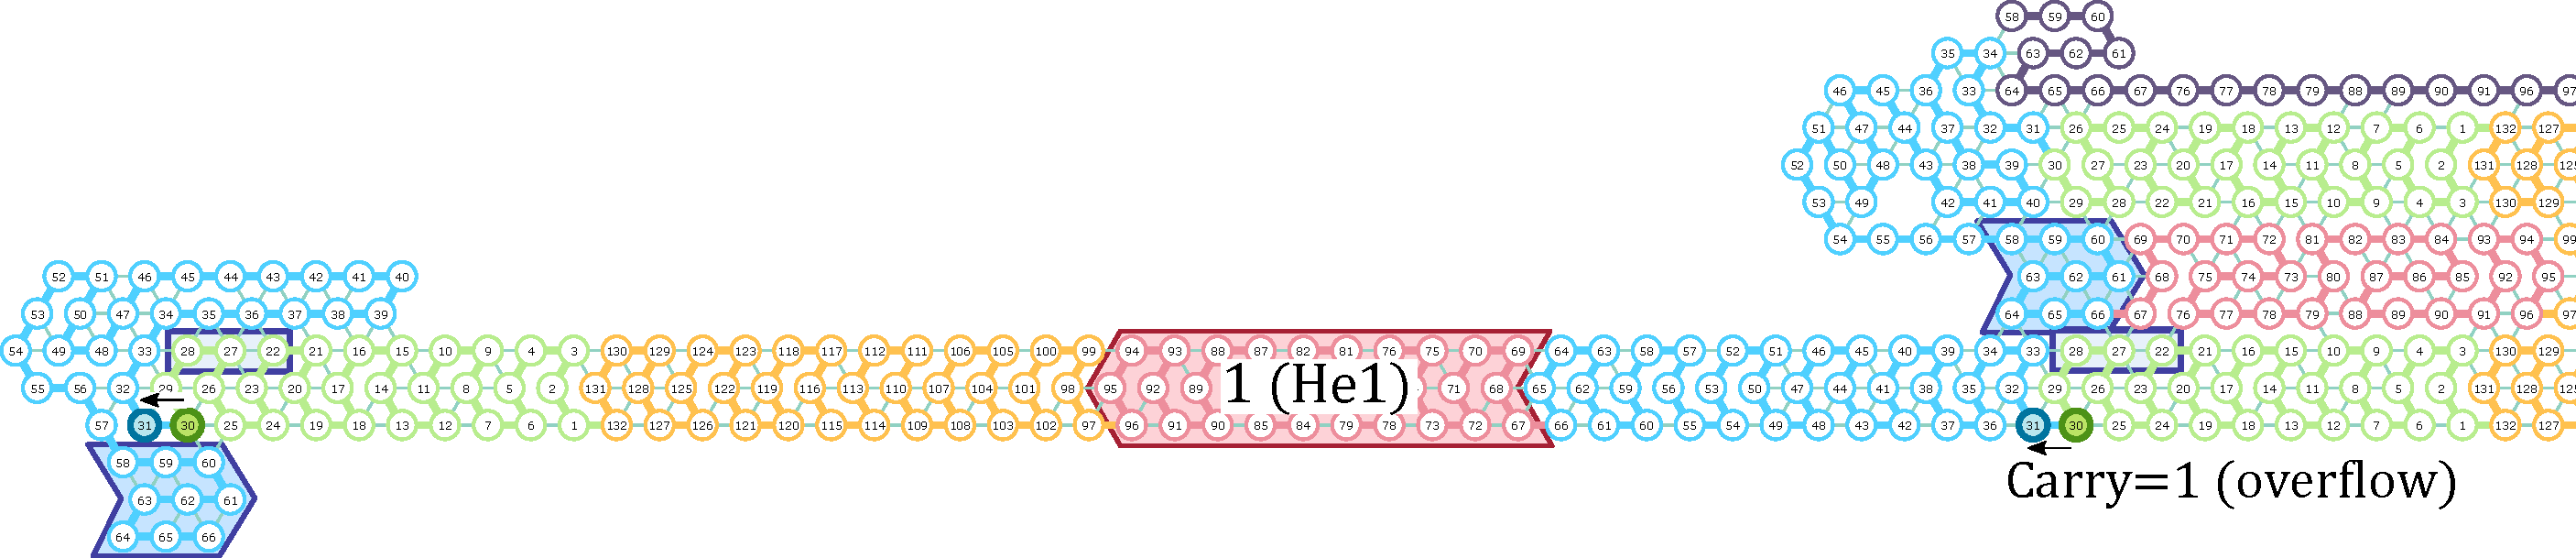
\includegraphics[width=\linewidth]{fig/svg/CounterEx18_1.pdf}
\caption{
Module L turns by module F's Turn Signal and zag pass starts.
Also, the end of L takes the form of Turn Signal.
}
\label{fig:overflowex5}
\end{figure}



% Lbeの後の話 Lcreまで
In the case of overflow, instance of H,  R, and F are transcribed following \texttt{Lbc} and they fold into \texttt{He1}, \texttt{Rb}, and \texttt{Fnb}, respectively.
Next instance of L which is transcribed after \texttt{Fnb} carriage-return for the next zag.
However, if its instance turn, Turn Signal must be present around there so the top of \texttt{Fnb} is given the role of Turn Signal.
Unless the count overflows, there is a brick above \texttt{Fnb} as shown in Fig.~\ref{fig:overflowex1}, so the top of \texttt{Fnb} is hidden, but when it overflows, Turn Signal is exposed.

Module H read from the row above the value encoded into folding in the module F during the previous zag-phase, and fold into a shape H00, H10, H01, H11.
H$xc$ is corresponding to the case where $x$ is the bit read in the row above and $c$ is the carry. 
In the zig pass module R, F, and L just propagate the carry value to the next.

When the zig pass reaches the left most part, module L collaborates with above turn module and it is folded turn module which reverses the folding direction for next zag pass except carry = 1.
At this time, if module L has a carry, folding of module L is glider and it go straight in order to expand bit width after that next module L turns to zag pass while folding turn module.
%H -> He1

\subsubsection{In the zag ($\rightarrow$)}
This part, instances of module F copy the current value, which incremented in the previous zig and encoded at below the zig.
Module F is always folded under module H in zags and F takes the two bricks F0 and F1 shown in Fig.~\ref{fig:formatters} which depending on a brick of module H.
Other modules H,R, and L take bricks which do nothing Hn, Rb, and Lbc, respectively, shown in Fig.~\ref{fig:halfadders}, \ref{fig:rightturns}, \ref{fig:leftturns}. 

a


Module F read form the row above H$xc$, and fold into a shape F0, F1.
F$y$ is corresponding to the case where $y = (x + c)$ mod $2$.
There are no carry propagation and the module L, H, R fold into Lbc, Hn, Rb in this pass.

When the zag pass reaches the right most part. module R collaborates with above turn module and it is folded turn module which reverses the folding direction for next zag pass.

\subsection{Example of folding first zigzag}
Let's run an infinite counter from 1 bit width.
The seed is encoded with "0", and the starts from bottom row, that is, giving a carry for the least significant bit.

\subsubsection{The first zig pass ($\leftarrow$)}
In Fig,~\ref{fig:counter1stzig}, the zig pass folds as follows.
\begin{itemize}
\item{[First module F (Light Green)]} \\Normally, module H is folded above module F, and the seed corresponding to this module H now represents None.
Then, module F forms a shape which represents None and propagates carry equal to 1.
\item{[First module L (Light Blue)]} \\Since the seed here does not have a turn signal, module L forms glider and propagates carry while extending straight.

\item{[First module H (Pink)]} \\The seed is encoded 0 and module folding starts from the bottom row, that is, the carry equal to 1.
Then, HA folds into H01, which represents 1 and is output of carry equal 0.

\item{[First module R (Yellow) and 2nd module F]} \\Both module form glider which start from top row and end to top row, in order to propagate carry equal 0.

\end{itemize}

\subsubsection{The first zag pass ($\rightarrow$)}
In Fig. \ref{fig:counter1stzig}, it is folded until second module F, and module L is transferred as the next transcript.
Fig. \ref{fig:counter1stzag} shows how zag pass is folded.
Now, there is a Turn Signal at the left end of the seed, so L's transcript binds to its signal and loses the shape of glider in order to turn.
In addition, the turned module L forms a Turn Signal at its end.

The zag pass folds as follows.
\begin{itemize}
\item{[module H and module R]} \\Since the module F of last module in zig pass represents None,
module H folds into Hn also representing None. The module R form glider for margin.
\item{[module F, L, and H]} \\There are three types of brick, H01, H10 and He1, representing 1 in module H, and different signals are defined as 1 any. Then, module F folds into brick F1 no matter which module H is above, representing 1. The module L folds glider and the module H folds brick Hn.

\end{itemize}



\subsection{Conformations of Module H}
The half adder module H forms five different paths as shown in Fig.~\ref{fig:halfadders} in zig pass.
Module H reads the already folded bead (F0 or F1) at above as one of the inputs, and determines the other input depending on the folding starts (top or bottom).
Module H forms four bricks of H00, H01, H10, and H11 for each input.
Then, the bricks outputs the sum as beads of bottom row and also outputs carry depending on whether module H is folded top or bottom except He1.
Brick He1 is the first folded module H after overflow.
Since this counter uses three row of gliders as a self-standing method, module H consisting of 30 beads has an even width, and when it starts folding from the bottom, folding ends at the bottom.
That is why brick He1 ends folding at the bottom and outputs carry equal to 0.

In the output sum, module H has 2 types of beads representing "0" and  3 types of beads representing "1".
Then, module F is folded to F0 and F1 in Fig.~\ref{fig:formatters} according to the beads corresponding to 0 (H00, H11) and 1 (H01, H10, He1), respectively, to format beads representing a value.




\subsection{Example of overflow}
Oritatami system proceeds to further fold the counter transcript form the state shown in Fig.~\ref{fig:counter1stzag}, it overflows (Fig.~\ref{fig:overflowex1}).
If it does not overflow, the next module L will bind to above Turn Signal and turn.
However, since the carry overflows, module L's folding starts from bottom row and does not reach Turn Signal, so L forms a self standing glider shape, goes straight and extends the zig pass (Fig.~\ref{fig:overflowex2}).
Then the folding of module H begins and this H also becomes a glider shape (Fig.~\ref{fig:overflowex3}).
There is nothing above the folded module H (brick He1), but the original value is recognized as "0" and He1 catches the carry.
However, the end of folding He1 is bottom row because He1 is glider, so for He1 only, the counter determins that the folding end position is bottom row as carry=0.
In this way, the infinite counter extends the bit width after it overflows.

Subsequently, module R and F are folded, and then module L folding starts (Fig.~\ref{fig:overflowex4}).
Since module L turns by binding to Turn Signal, it is necessary to give signal for turn in order to move to zag pass from here.
Therefore, let the top of folded module F be Turn Signal.
Normally, there are folded beads above module F, so module L can not bind to F's Turn Signal.
However, only when it overflows, above F becomes blank, so L turns by being folded there (Fig.~\ref{fig:overflowex5}).
The turned module L forms a Turn Signal at the end, and folding of zag pass starts.


\subsection{Conformations of Module L}
The left turn module L forms five different paths as shown in Fig~\ref{fig:leftturns}.
In normal zig zag folding, module L is a glider like Lt or Lbc, but when transcript of L binding to Turn Signal, it formed as a turn module like Ltrc or Ltre.
Module L in the form as turn module has Turn Signal in its ends and it helps other L turn at the next zig-zag.
In zig pass, when module L reaches the left end, if it does not overflow, it bind to this Turn Signal and turned.
If module L overflows, it forms Lbe and continues the zig pass.
Then, module L which is folded next to Lbe, forms Ltre and turns by binding to the top of module F that is just before it.
At this time, the top of module F functions as Turn Signal, but this is the behavior only overflow because otherwise there is some folded module above module F.

\section{The brick automaton}
Beads which has already been folded around, that is, the environment decide which module transcript will be.
The environmental transition is represented Fig.~\ref{fig:brickautomaton}.
In addition, each symbol written as a state transition is conformation such as Fig.~\ref{fig:transitionconformation}
%\centering
%\begin{table}[tb]
%\begin{tabular}{c c c c}
%\begin{minipage}{25mm}
%	\centering
%       \scalebox{0.5}{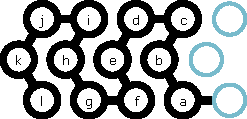
\includegraphics{fig/svg/bglider.pdf}}
%\end{minipage} &
%\begin{minipage}{25mm}
%	\centering
%       \scalebox{0.5}{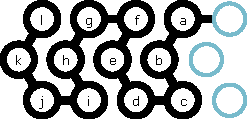
\includegraphics{fig/svg/tglider.pdf}}
%\end{minipage} &
%\begin{minipage}{30mm}
%	\centering
%       \scalebox{0.5}{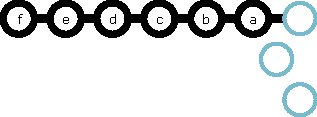
\includegraphics{fig/svg/plane.pdf}}
%\end{minipage} &
%\begin{minipage}{25mm}
%	\centering
%       \scalebox{0.5}{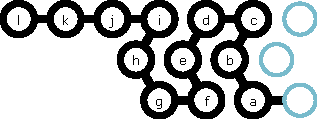
\includegraphics{fig/svg/spiral.pdf}}
%\end{minipage}\\
%
%\begin{minipage}{25mm}
%	\centering
%       \scalebox{0.5}{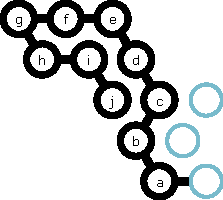
\includegraphics{fig/svg/horn.pdf}}
%\end{minipage} &
%\begin{minipage}{30mm}
%	\centering
%       \scalebox{0.5}{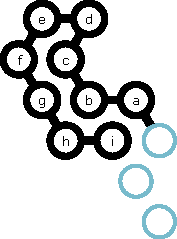
\includegraphics{fig/svg/kar.pdf}}
%\end{minipage} &
%\begin{minipage}{25mm}
%	\centering
%       \scalebox{0.5}{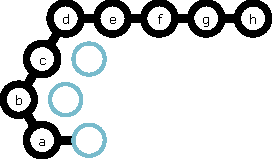
\includegraphics{fig/svg/roof.pdf}}
%\end{minipage}\\
%
%\begin{minipage}{25mm}
%	\centering
%       \scalebox{0.5}{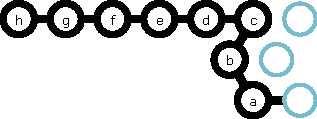
\includegraphics{fig/svg/fault.pdf}}
%\end{minipage} &
%\begin{minipage}{30mm}
%	\centering
%       \scalebox{0.5}{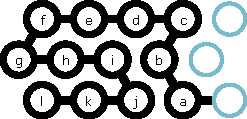
\includegraphics{fig/svg/cliff.pdf}}
%\end{minipage}\\
%
%\end{tabular}
%\end{table}

\begin{figure}[tb]
\centering
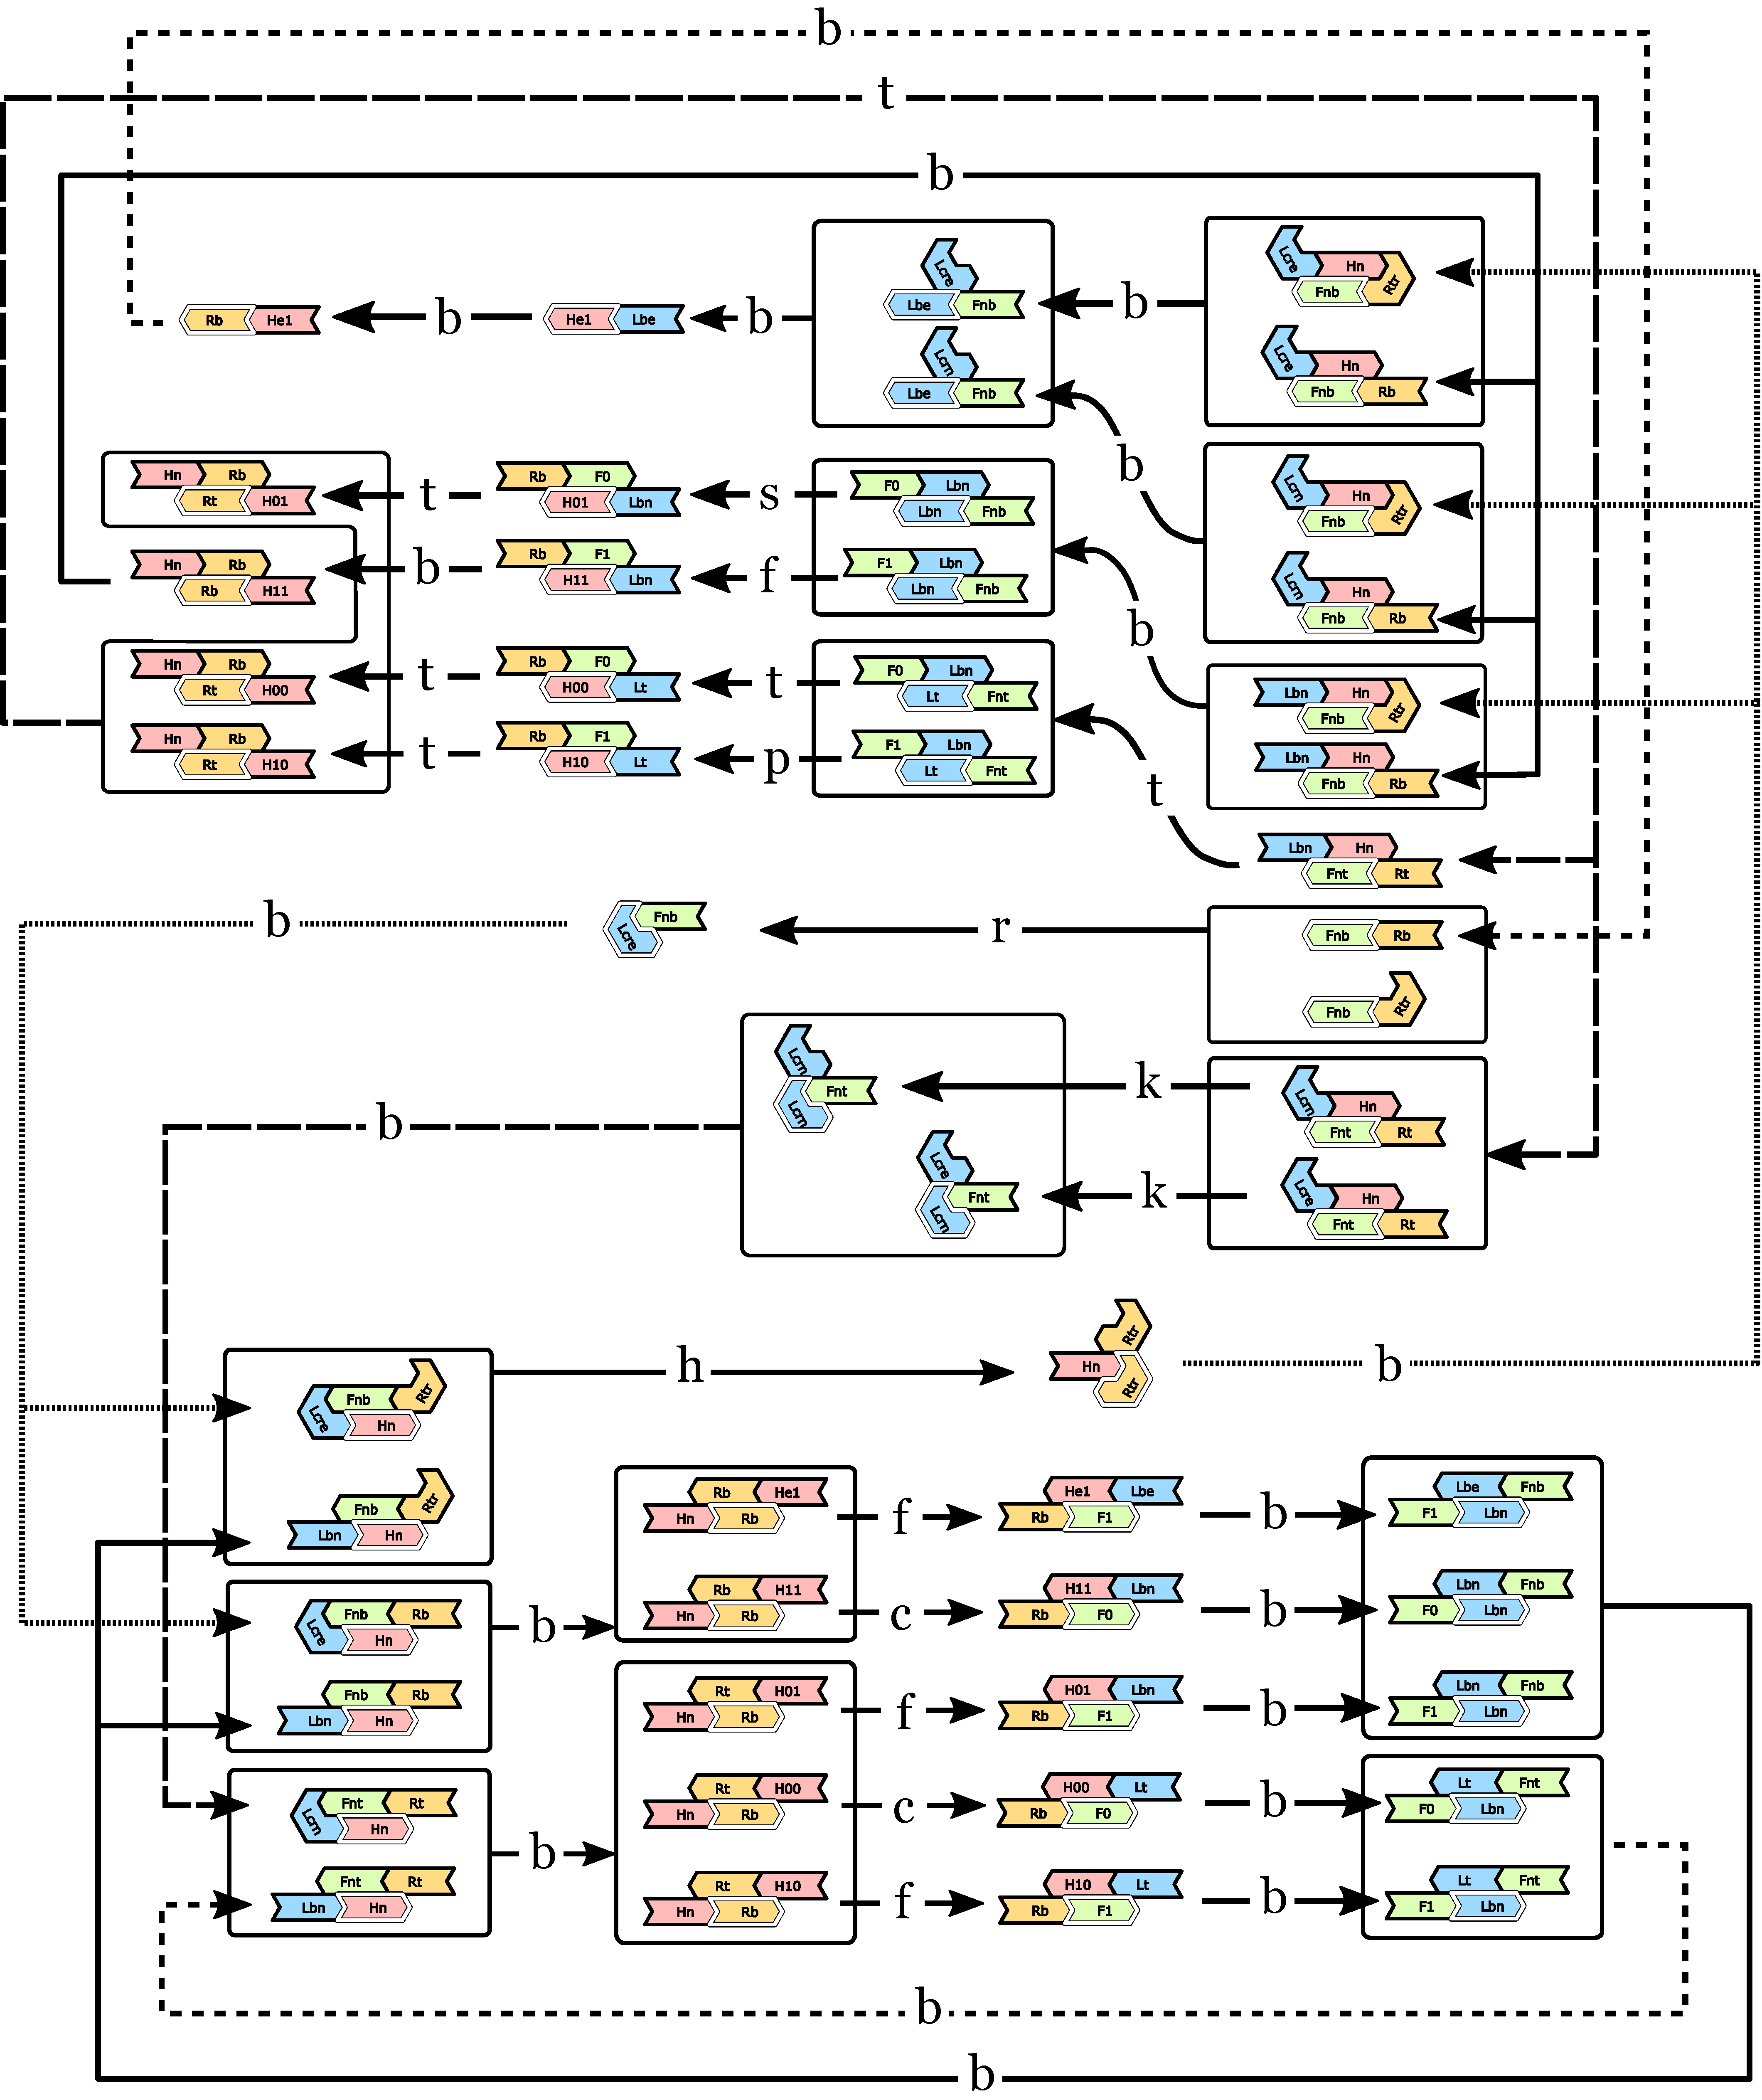
\includegraphics[width=\textwidth]{fig/svg/inf-ai_c_2.pdf}
\vspace*{5mm}

\scalebox{0.8}{
\begin{tikzpicture}
	\node[anchor=north, inner sep=0] (tg) at (0,0) {
 		   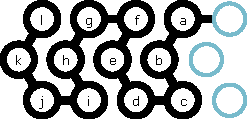
\includegraphics[width=0.2\textwidth]{fig/svg/tglider.pdf}
	};
	\node[anchor=north, inner sep=0] (bg) at (3,0) {
 		   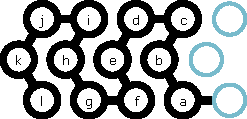
\includegraphics[width=0.2\textwidth]{fig/svg/bglider.pdf}
	};
	\node[anchor=north, inner sep=0] (pl) at (6,0) {
 		   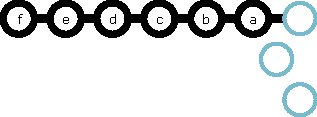
\includegraphics[width=0.2\textwidth]{fig/svg/plane.pdf}
	};
	\node[anchor=north, inner sep=0] (sp) at (9,0) {
 		   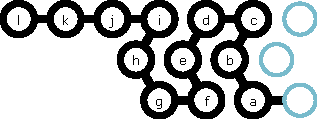
\includegraphics[width=0.2\textwidth]{fig/svg/spiral.pdf}
	};
	
	\node[anchor=north, inner sep=0] (ho) at (-1.5,-3) {
 		   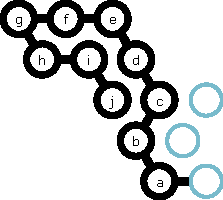
\includegraphics[width=0.2\textwidth]{fig/svg/horn.pdf}
	};
	\node[anchor=north, inner sep=0] (ka) at (1.5,-3) {
 		   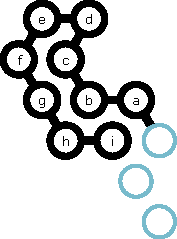
\includegraphics[width=0.15\textwidth]{fig/svg/kar.pdf}
	};
	\node[anchor=north, inner sep=0] (ro) at (4.5,-3) {
 		   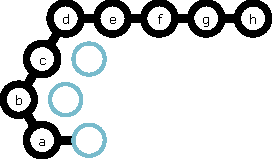
\includegraphics[width=0.2\textwidth]{fig/svg/roof.pdf}
	};
	\node[anchor=north, inner sep=0] (fa) at (7.5,-3) {
 		   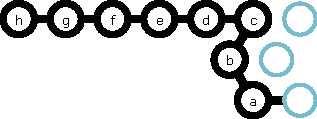
\includegraphics[width=0.2\textwidth]{fig/svg/fault.pdf}
	};
	\node[anchor=north, inner sep=0] (ci) at (10.5,-3) {
 		   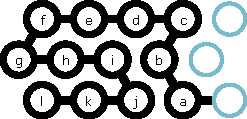
\includegraphics[width=0.2\textwidth]{fig/svg/cliff.pdf}
	};
	
	\node[below, shift=(-90:0.8)] at (tg) {t};
	\node[below, shift=(-90:0.8)] at (bg) {b};
	\node[below, shift=(-90:0.8)] at (pl) {p};
	\node[below, shift=(-90:0.8)] at (sp) {s};

	\node[below, shift=(-90:1)] at (ho) {h};
	\node[below, shift=(-90:1)] at (ka) {k};
	\node[below, shift=(-90:0.8)] at (ro) {r};
	\node[below, shift=(-90:0.8)] at (fa) {f};
	\node[below, shift=(-90:0.8)] at (ci) {c};
\end{tikzpicture}
}
%\caption{Transition conformations}
%\label{fig:transitionconformation}
%\end{figure}


%\begin{figure}[tb]
\caption{The brick automaton of infinite binary counter}
\label{fig:brickautomaton}
\end{figure}

\begin{thebibliography}{1}

\bibitem{AdChGoHu2001}
Leonard Adleman, Qi Chang, Ashish Goel, and Ming-Deh Huang, 
Running time and program size for self-assembled squares, 
In Proc. STOC 2001, ACM, 740-748, 2001. 

\bibitem{BrChDoKaSe2013}
Nathaniel Bryans, Ehsan Chiniforooshan, David Doty, Lila Kari, and Shinnosuke Seki, 
The power of nondeterminism in self-assembly, 
\textit{Theory of Computing}, vol. 9, 1-29, 2013.

\bibitem{EvansPhD}
Constantine Glen Evans, 
Crystals that Count! Physical Principles and Experimental Investigations of {DNA} Tile Self-Assembly, 
Ph.D. thesis, Caltech, 2014.

\bibitem{GeMeScSe2019}
Cody Geary, Pierre-\'{E}tienne Meunier, Nicolas Schabanel, and Shinnosuke Seki, 
Oritatami: A computational model for molecular co-transcriptional folding, 
\textit{International Journal of Molecular Sciences} vol. 20(9), 2259, 2019. Its conference version was published in Proc. MFCS 2016. 

\bibitem{GearyRothemundAndersen2014}
Cody Geary, Paul W. K. Rothemund, and Ebbe S. Andersen, 
A single-stranded architecture for cotranscriptional folding of {RNA} nanostructures, 
\textit{Science} vol 345(6198), 799-804, 2014.

\bibitem{MasudaSekiUbukata2018}
Yusei Masuda, Shinnosuke Seki, and Yuki Ubukata, 
Towards the algorithmic molecular self-assembly of fractals by cotranscriptional folding, 
In Proc. CIAA 2018, LNCS 10977, Springer, 261-273, 2018.

\bibitem{McClung2006} 
C. Robertson McClung, 
Plant circadian rhythms, 
\textit{The Plant Cell}, vol. 18, 792-803, 2006.

\bibitem{Minsky1967}
Marvin Minsky, 
Computation: Finite and Infinite Machines, 
Prentice-Hall, Inc., 1967. 

\bibitem{RothemundWinfree2000}
Paul W. K. Rothemund and Erik Winfree, 
The program-size complexity of self-assembled squares (extended abstract), 
In Proc. STOC 2000, ACM, 459-468, 2000.

\bibitem{WinfreePhD}
Erik Winfree, 
Algorithmic Self-Assembly of {DNA}, 
Ph.D. thesis, Caltech, 1998.

\bibitem{GeMeScSe2018}
Cody Geary and Pierre-\'Etienne Meunier and Nicolas Schabanel and Shinonsuke Seki,
Proving the {T}uring Universality of Oritatami Cotranscriptional Folding,
Proc. ISAAC 2018,
23:1 -- 23:13,2018.


\end{thebibliography}
  
\end{document}
